\documentclass{ieeeojies}
\usepackage{cite}
\usepackage{amsmath,amssymb,amsfonts}
\usepackage{algorithmic}
\usepackage{graphicx}
\usepackage{textcomp}
\usepackage{listings}
\usepackage{todonotes}
%\usepackage[table]{xcolor}
\usepackage[most]{tcolorbox}
\usepackage{url}
\newtcolorbox{rquestion}[1]{colback=gray!5!white,colframe=gray!75!black,fonttitle=\bfseries,title={#1},left=1mm,right=1mm, top=1mm, bottom=1mm}    

\newtcolorbox{rdirection}{leftrule=2mm,colback=gray!5!white,colframe=gray!75!black,left=1mm,right=1mm, top=1mm, bottom=0mm}


\def\BibTeX{{\rm B\kern-.05em{\sc i\kern-.025em b}\kern-.08em
    T\kern-.1667em\lower.7ex\hbox{E}\kern-.125emX}}
\begin{document}


%\title{Generating Portable Test Cases for IEC~61499 FBs from Interface Behaviour Specifications}
%\title{A Test Framework for Cross-Platform Development of IEC~61499-based Control Software}
\title{Develop Once, Test Everywhere: Cross-Platform Development of Distributed Control Software}

\author{
\uppercase{Bianca Wiesmayr}\authorrefmark{1},
\uppercase{Melanie Winter}\authorrefmark{1},
\uppercase{Midhun Xavier}\authorrefmark{2},
\uppercase{Sandeep Patil}\authorrefmark{2},
\uppercase{Valeriy Vyatkin}\authorrefmark{2,4} \IEEEmembership{Fellow, IEEE},
\uppercase{and Alois Zoitl}\authorrefmark{3} \IEEEmembership{Senior Member, IEEE}}

\address[1]{LIT CPS Lab, Johannes Kepler University Linz, Austria (e-mail: bianca.wiesmayr@jku.at)}
\address[2]{Luleå University of Technology, Luleå, Sweden (e-mails: midhun.xavier@ltu.se, sandeep.patil@ltu.se)}
\address[3]{CDL VaSiCS, LIT CPS Lab, Johannes Kepler University Linz, Austria (e-mail: alois.zoitl@jku.at)}
\address[4]{Aalto University, Helsinki, Finland (e-mail: Valeriy.Vyatkin@aalto.fi)}

\tfootnote{This work was sponsored in part by the Horizon Europe project Zero-SWARM funded by the European Commission (grant agreement: 101057083).}

\corresp{Corresponding author: Valeriy Vyatkin (e-mail: Valeriy.Vyatkin@aalto.fi).}

\begin{abstract}
IEC 61499 is an executable event-based language for control software that allows visual and textual implementation of individual software components, so-called Function Blocks (FBs). In heterogeneous environments, relevant features are the transfer of software and libraries between tools (portability) and the configuration of multiple runtime environments from a single IDE (configurability). Due to ambiguities and deviations from the standard, the FB behaviour slightly varies on each available platform. Such variations are not only observed in IEC~61499-based software and limit portability in practice. This paper therefore investigates an approach for software testing which involves generating portable test code from a specification model. For cross-platform validation, the test code is executed in each relevant run-time environment. We have evaluated our approach in a test-driven development process for a drilling demonstrator. Eclipse 4diac was extended to automatically generate the test code, which was subsequently ported to another IDE. The generation mechanisms consider platform-specific deviations from the IEC~61499-standard to promote portability. We demonstrated the feasibility of cross-platform testing for IEC~61499-based components, enabling further work in the area of test case generation.


\begin{comment}
Hence, executing FB tests in the target platform helps validate the correct functionality of an FB. % before deploying control software to a cyber-physical system. 
%The standardized visual service sequence model 
Interface models in IEC 61499 specify the expected input/output behaviour of a component. A test execution framework can use this information for model-based testing, but these tests are currently not portable. %However, the available approaches require the use of a certain development environment and do not allow specifying tests for control software in a platform-independent way.
In this paper, we use the modelled tests to automatically generate a platform-independent test application that allows validating the functionality of an FB on various platforms. The test automation helps detect any relevant variations in execution behavior among platforms. 
%First, service sequences as test specifications are generated manually or are derived from an existing (partial) implementation. They serve as unit tests for these FBs. We generate a complete 
The test application that is executable on any IEC 61499-compliant platform and automatically compares the results obtained from the FB under test with the expected results. After generation, the test code is fully compliant with the IEC~61499-standard and does not rely on any tool-specific extensions. Hence, it can be ported between platforms. We have evaluated our approach using a test suite as well as a set of FBs that control a demonstrator. We used two IEC~61499 platforms, Eclipse 4diac and SE EcoStruxure, to evaluate the portability of the generated test application. The generation approach takes into account any platform-specific deviations from the IEC~61499-standard. In order to further promote portability between platforms, we also list deviations from the IEC standard for each platform.
\end{comment}
\end{abstract}

\begin{keywords}
Model-based Testing, IEC 61499, Function Blocks, Service Sequences, Portability
\end{keywords}

%\titlepgskip=-15pt
\setlength{\titlepgskip}{-15pt}

\maketitle

\section{Introduction}
\label{sec:introduction}
Realising flexible industrial automation systems requires an approach
 for autonomous and distributed designs \cite{Lyu.2021}. Programmable Logic Controllers (PLCs) are the established platform for real-time control software that accesses sensors and actuators \cite{Sehr.2021}.  Standards play an important role in distributed automation, for instance, IEC~61131-3 and IEC~61499, which define programming paradigms for control software development \cite{Lyu.2021}. %Despite the increasing complexity of automation systems, the programming models of IEC 61131-3 are still prevalent \cite{Sehr.2021}. 
 Multiple interacting PLCs form a distributed control system. Providing the respective engineering methodologies and models is a goal of IEC~61499 \cite{61499}. Heterogeneous systems can even be composed of PLCs from various vendors and programmed with different tools \cite{lyu2020towards} \cite{mazzolini2017structured}. Furthermore, a single development tool can distribute control code across multiple runtime environments (RTEs)~\cite{eclipse4diac}, motivating the need to execute component tests in each of these RTEs. Developers of IEC~61499 library modules  \cite{oberlehner.2022} will also need to provide their modules to users of various development environments. 
 Despite the focus on portability \cite{61499} and the standardized XML format for data exchange \cite{61499.2}, IEC~61499-based software components must often be modified during the porting process \cite{Hopsu.2019, Testing_Midhun}. Due to varying execution behaviour, the ported software may behave differently on each platform \cite{Testing_Midhun, Wiesmayr.2023}, possibly leading to malfunctions of the distributed control system. Therefore, it is crucial to thoroughly test an IEC 61499 application on each relevant target platform before using the software in a real-world system. A platform-independent test specification has the potential to greatly reduce the involved effort.
\begin{figure*}[t]
    \centering
    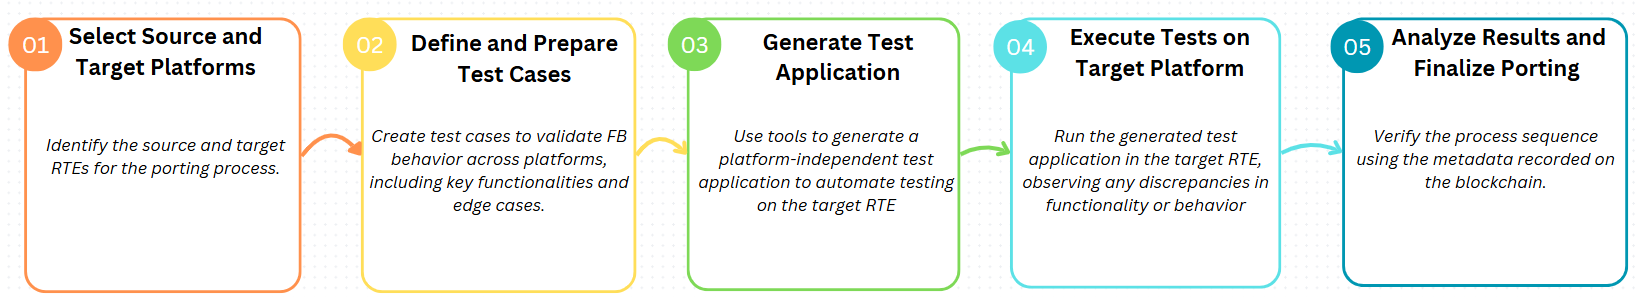
\includegraphics[width=0.95\linewidth]{OJIES_2024/Figures/portingProcessPNG.PNG}
    \caption{Process of porting test code for IEC~61499 Function Blocks between execution environments.}
    \label{fig:porting_process}
\end{figure*}
%The IEC 61499 standard \cite{61499} addresses the issues of vendor lock-in and offers a solution by providing a framework for developing portable and interoperable software. Although the file exchange format is standardised, it is currently interpreted differently and the execution behavior varies among vendors \cite{christensen.2012,Thramboulidis.2009}. 

%\todo[inline]{MX: add references and details, paragraph is complicated to read}
Evaluating a system's correctness typically involves providing test data and observing the system's reaction. Such tests are specified manually, obtained from models, or generated using other techniques \cite{Sinha.2019}. The engineering processes of complex control systems additionally require that PLC platforms ensure reliability through simulation and verification, rather than relying on iterative testing of a cyber-physical system \cite{Sehr.2021}. Simulation methods evaluate only a system model and, thus, can provide results faster \cite{Sinha.2019}. In the context of IEC~61499, executing test cases within a run-time environment can be considered a simulation. A certain degree of test automation is required to efficiently evaluate this software. Existing test processes for IEC~61499-based software rely on a framework in the target platform (e.g., \cite{hametner2014}) and are therefore not applicable for cross-platform development of IEC~61499-based software. When (re-)using parts of IEC~61499 software in multiple platforms, extensions to the IEC~61499 standard may not be available in all platforms (equally). Hence, we are investigating an approach for test automation that does not require any extensions of IEC~61499.

% Current control systems are highly dependent on specific vendors, hindering the transfer of programs between different platforms \cite{}. As seamless integration is a key requirement in the context of Industry 4.0, this lack of portability poses great challenges \cite{}.

%As a result, migrating programs from one IEC 61499 platform to another, and thus executing them in a different run-time environment (RTE), may introduce errors that are difficult to detect but could lead to damage to humans or the physical equipment \cite{Testing_Midhun}. Therefore, it is crucial to thoroughly test an IEC 61499 application on the target platform before deploying it to a real-world system. A platform-independent test specification has the potential to greatly reduce the involved effort.
\begin{rquestion}{Research Question (RQ)}
    How can we automate the testing of IEC 61499 software components to evaluate their correct behaviour across platforms from different vendors?
\end{rquestion}

This paper aims to address the challenge of evaluating the effect of porting software components to other platforms or configuring additional RTEs. The test framework allows us to execute tests in any IEC~61499-compliant RTE. Based on our initial concept presented in \cite{biancaMidhunETFAwip}, we generate an IEC~61499-compliant test application that automatically provides test events and data, compares the results of the software component under test with the expected observable behaviour and summarises the results so that they are accessible by the user. The general process is visualised in Figure~\ref{fig:porting_process}. 
Like Hametner et al.~\cite{hametner2014}, we use service sequence models as test specifications. Related work in the context of testing and porting IEC~61499 components is outlined in Section~\ref{sec::sota}. Section~\ref{sec::running_example} introduces a running example. Based on this example, Section~\ref{sec::methodology} outlines the envisioned methodology to test FBs on any IEC~61499-compliant platform. 
One of these IDEs, the 4diac IDE from the Eclipse 4diac open source project, was extended to generate the test application. 
The generation rules for a test application and their implementation are described in Section~\ref{sec::implementation}. Realised as a composite FB, the test application is portable across various IEC 61499 platforms and enables validation of the correct functionality before deployment in real-world machinery. We evaluated our approach using a demonstrator (Section~\ref{sec::casestudy}). Section~\ref{sec::results} lists the identified portability issues and programming errors that we could detect using our test suite. In addition, we discuss limitations of our approach before concluding our paper in Section~\ref{sec::conclusions}. 


%Previous work showed the feasibility of using service sequences as test specifications \cite{wiesmayr2021,hametner2014}. 
%Existing testing mechanisms require dedicated tool support and cannot be directly transferred to other platforms. The portability of IEC 61499 software allows migrating applications to other IEC 61499 vendor platforms, but ensuring that a program behaves consistently across RTEs remains an open challenge. 
%In this paper, we therefore present our approach for testing FBs that allows to execute tests on any IEC 61499-compliant RTE. Based on test scenarios that are created as a service sequence model, we generate the corresponding test application. %FB, establish the necessary connections with the FB under test, execute each test scenario, compare the results, and provide the test outcome. 
\section{Related Work}
\label{sec::sota}

Portability, interoperability, configurability, and distribution across devices are key goals of IEC~61499 \cite{jhunjhunwala2024interoperability,hopsu2019portability, batchkova2013dynamic}. 
This has led to its application in use cases of flexible manufacturing systems, such as multi-agent systems \cite{lyu2023multi, xavier2024enhancing}. However, portability between vendors has not yet been achieved due to vendor-specific execution behaviour \cite{misperceptions}. In this section, we therefore review recent studies on porting software between engineering platforms. Furthermore, techniques for improving the reliability of control software are discussed with a focus on testing approaches. The approach proposed in this paper aims to test software components on different platforms, thus, promoting reusability of software as well as supporting the process of porting software components. 

\subsection{Portability of Control Software}
Both standards that define programming languages for control software, i.e., IEC~61131-3 \cite{61131.3} and IEC~61499-1 \cite{61499}, define XML formats for exchanging software between PLC environments \cite{61131.10,plcopenpaper, 61499.2, Testing_Midhun}. The standardised format contributes to code exchange between tools from different vendors~\cite{plcopenpaper}. As existing tools only support a varying subset of features, portability is limited in practice \cite{Testing_Midhun}. Certain vendors also use custom XML tags to store additional information in their projects which are not covered by the standard itself, such as namespaces in IEC~61499. The resulting software may still be portable if the parser in the target IDE discards unknown XML tags that carry additional information \cite{Hopsu.2019}.  The language specification focusses on control software without detailing applied communication standards or visualisation options. Language extensions, such as modelling elements for communication \cite{Bruns.2023}, are not widely supported and therefore not yet portable. One of the IDEs allows specifying the human-machine interaction (HMI) as part of the control code with dedicated blocks, so-called CAT elements \cite{Hopsu.2019}. Converter programs can help translate programs between syntactic variants of IEC~61499 \cite{Hopsu.2019}, but vendor-specific extensions can typically not be transferred. 
Even syntactic equivalence does not guarantee portability. Nowadays, cross-platform development does not require porting because a single IDE allows deploying software to multiple run-time environments \cite{aimirimi}. 
The IEC~61499 language semantics is not specified formally and is subject to interpretation. Different execution semantics have emerged, which can affect the behaviour of the cyber-physical system \cite{cengic_executionsemantics}. Hence, migrating IEC~61499-based software to different run-time environments can introduce errors that may cause damage to operators or equipment. While the syntactic portability has been addressed \cite{Hopsu.2019,Testing_Midhun}, different execution behaviours cannot yet be detected (semi-)automatically. It is therefore crucial to thoroughly test IEC~61499 applications in the target platform before deployment. Existing testing mechanisms enable systematically evaluating the implemented execution semantics of IEC~61499 runtime environments \cite{Wiesmayr.2023,pfefferkorn,Testing_Midhun}, but a solution for porting test cases including their execution framework to different platforms is not yet available. We have presented our initial concept in \cite{biancaMidhunETFAwip}. 

%%%%%%%%%%%%%%%%%%%%%%%%%%%%%%%%%%%%%%%%%%%%%%%%%%%%%%%
\subsection{Validating Control Software}
%\todo[inline]{Add references and details}
Cengic and Akesson~\cite{cengic_executionsemantics} followed the approach of creating a formal semantics specification for each runtime environment. Subsequently, formal verification methods can be applied to identify errors in the code \cite{xavier2024framework}, which can enhance a system's reliability by checking various properties. Formal verification does not require access to any RTE, but a model of the execution behaviour is required. Sinha et al.~\cite{Sinha.2019} provide an overview of formal methods for IEC~61499. Formal verification may uncover errors that do not occur during simulations, thus, identifying certain undesirable situations \cite{lilli2023formal}. 
Control software has to be continuously adapted to changing requirements. Research has therefore provided guidance on the correct evolution of control software developed in IEC~61499 \cite{faqrizal_guidedevolution}. 
Verification and testing can complement each other \cite{Hussain.2006}. During development, tests provide early feedback, even if the model is still incomplete. Furthermore, errors that are introduced during the deployment may lead to issues encountered during runtime, but might not be revealed by formal methods \cite{ovsiannikova2023formal} \cite{xavier2023formal}. Hence, testing deployed software directly in the run-time environment remains valuable.
%Simulation techniques such as visualisations or Digital Twins are commonly employed to assess whether a control application operates according to the intended logic. However, relying on a simulation does not ensure correctness, as some malfunctions may occur only on a PLC. Finally, simulations can also aid in comprehending the system's behaviour.

Developers can apply various testing strategies, which we differentiate based on the involved software activities (e.g., unit tests or integration tests), the maturity of the software, and the degree of automation~\cite{softwareTesting}. 
Unit testing is a fundamental approach to software testing, which evaluates the implementation of a piece of software \cite{softwareTesting} to ensure software reliability.
In IEC~61499, the relevant units are individual Function Blocks (FBs) \cite{hametner2014}. Executing a test requires providing event and data signals. For control engineers who develop FBs, it can be challenging to manually create a test FB and the required test application, which derives and collects the test results. Model-based testing can reduce manual effort and also supports a ``test first and fail'' methodology, known as Test-Driven Development (TDD) \cite{hametner2014}, which is used in agile software engineering.  
After developing the control program for the entire system, functional tests can be conducted. This involves evaluating the control system by providing input data and verifying the output against expected results.

Tools should support engineers in specifying test cases to reduce the required software engineering knowledge and increase efficiency \cite{hametner2014}. Model-based testing involves automating at least part of the testing activities. For IEC~61499 FBs, service sequences are suitable for specifying tests \cite{hametner2014}. 
% TODO describe here in related work existing work on model-based testing or sth like that?? shift our new work to the beginning of the next section
A test runner can execute these tests in an RTE and automatically evaluate the results \cite{hametner2014}. Additionally, executing models directly can allow feedback without involving any RTE and is also feasible for service sequences \cite{wiesmayr2021}. The former approach requires specific tool support for a certain RTE, the latter cannot provide feedback regarding issues introduced in the deployment to an RTE. Our approach builds upon these works. 
As an alternative to service sequences, UML models have been used as test specifications \cite{Hussain.2006}. From a state-based model, test cases can be derived using coverage-driven algorithms \cite{Hussain.2006}. Using an evolutionary algorithm, test cases with a high coverage were generated directly from the FB model in \cite{Buzhinsky.2015}. Test case generation can augment our approach, which focusses on executing tests of any source on multiple platforms. Additional tool support would be required to use other test specifications than service sequences.
%In this approach, a test specification is created as service sequences to test the developed IEC 61499 function block with control logic. However, this approach is executed in the interpreter and does not have runtime support. The results are compared to the output of the sequence primitive.

Two major problems are still associated with developing distributed control software that spans multiple platforms: 
\begin{itemize}
    \item The \emph{lack of automated tool support for RTE comparison} makes comparing the behaviour and performance of FBs across different RTEs a challenging task. Currently, manual comparison is time-consuming and error-prone. Dedicated tools should analyse and evaluate the behaviour of FBs in different RTEs to ensure an accurate comparison.
    \item \emph{Software development for different RTEs} is challenging because the compatibility and portability of an FB across different RTEs cannot be assumed.
\end{itemize}
For example, if an FB is initially developed and tested on one RTE, such as SE EcoRT, there might be a need to reuse that FB in another project in a different RTE, such as 4diac FORTE. Differences in RTE behaviour, programming languages, and underlying architectures can cause compatibility issues and hinder the seamless transfer of FBs between different RTEs. 

\subsection{Cross-Platform Tests of Control Software}
Two main strategies are relevant for IEC~61499-based software. Firstly, \textbf{manually created test FBs} \cite{Testing_Midhun} can reveal the behaviour implemented in an RTE. Each test FB encompasses multiple test scenarios and embeds control logic. To indicate whether a test was successful, the expected result is compared with the result obtained from executing the control logic. The tests are implemented as a Basic FB with event and data pins. Each input event represents a test scenario linked to specific data inputs, while output events indicate the expected result and corresponding data outputs. When a test scenario is triggered, the state diagram (i.e., Execution Control Chart, ECC) executes an algorithm that assigns input values, generates outputs based on those values, and triggers the output event. The main purpose of these FBs was to identify differences between the execution behaviour in RTEs, not to test FB libraries. Similarly, small networks of FBs can further expand these test suites \cite{pfefferkorn,Wiesmayr.2023}. 
As a second approach, \textbf{generating test code from a high-level test specification} has the potential to enable testing FB implementations \cite{biancaMidhunETFAwip}.
\section{Running Example: Simple Calculation FB}
\label{sec::running_example}
As a running example, we use an FB that performs a simple calculation (Figure~\ref{fig:running_example}) based on the inputs according to the formula \texttt{DO1:=DI1+2*DI2}. It contains the following language elements:

\begin{figure}[b]
    \centering
    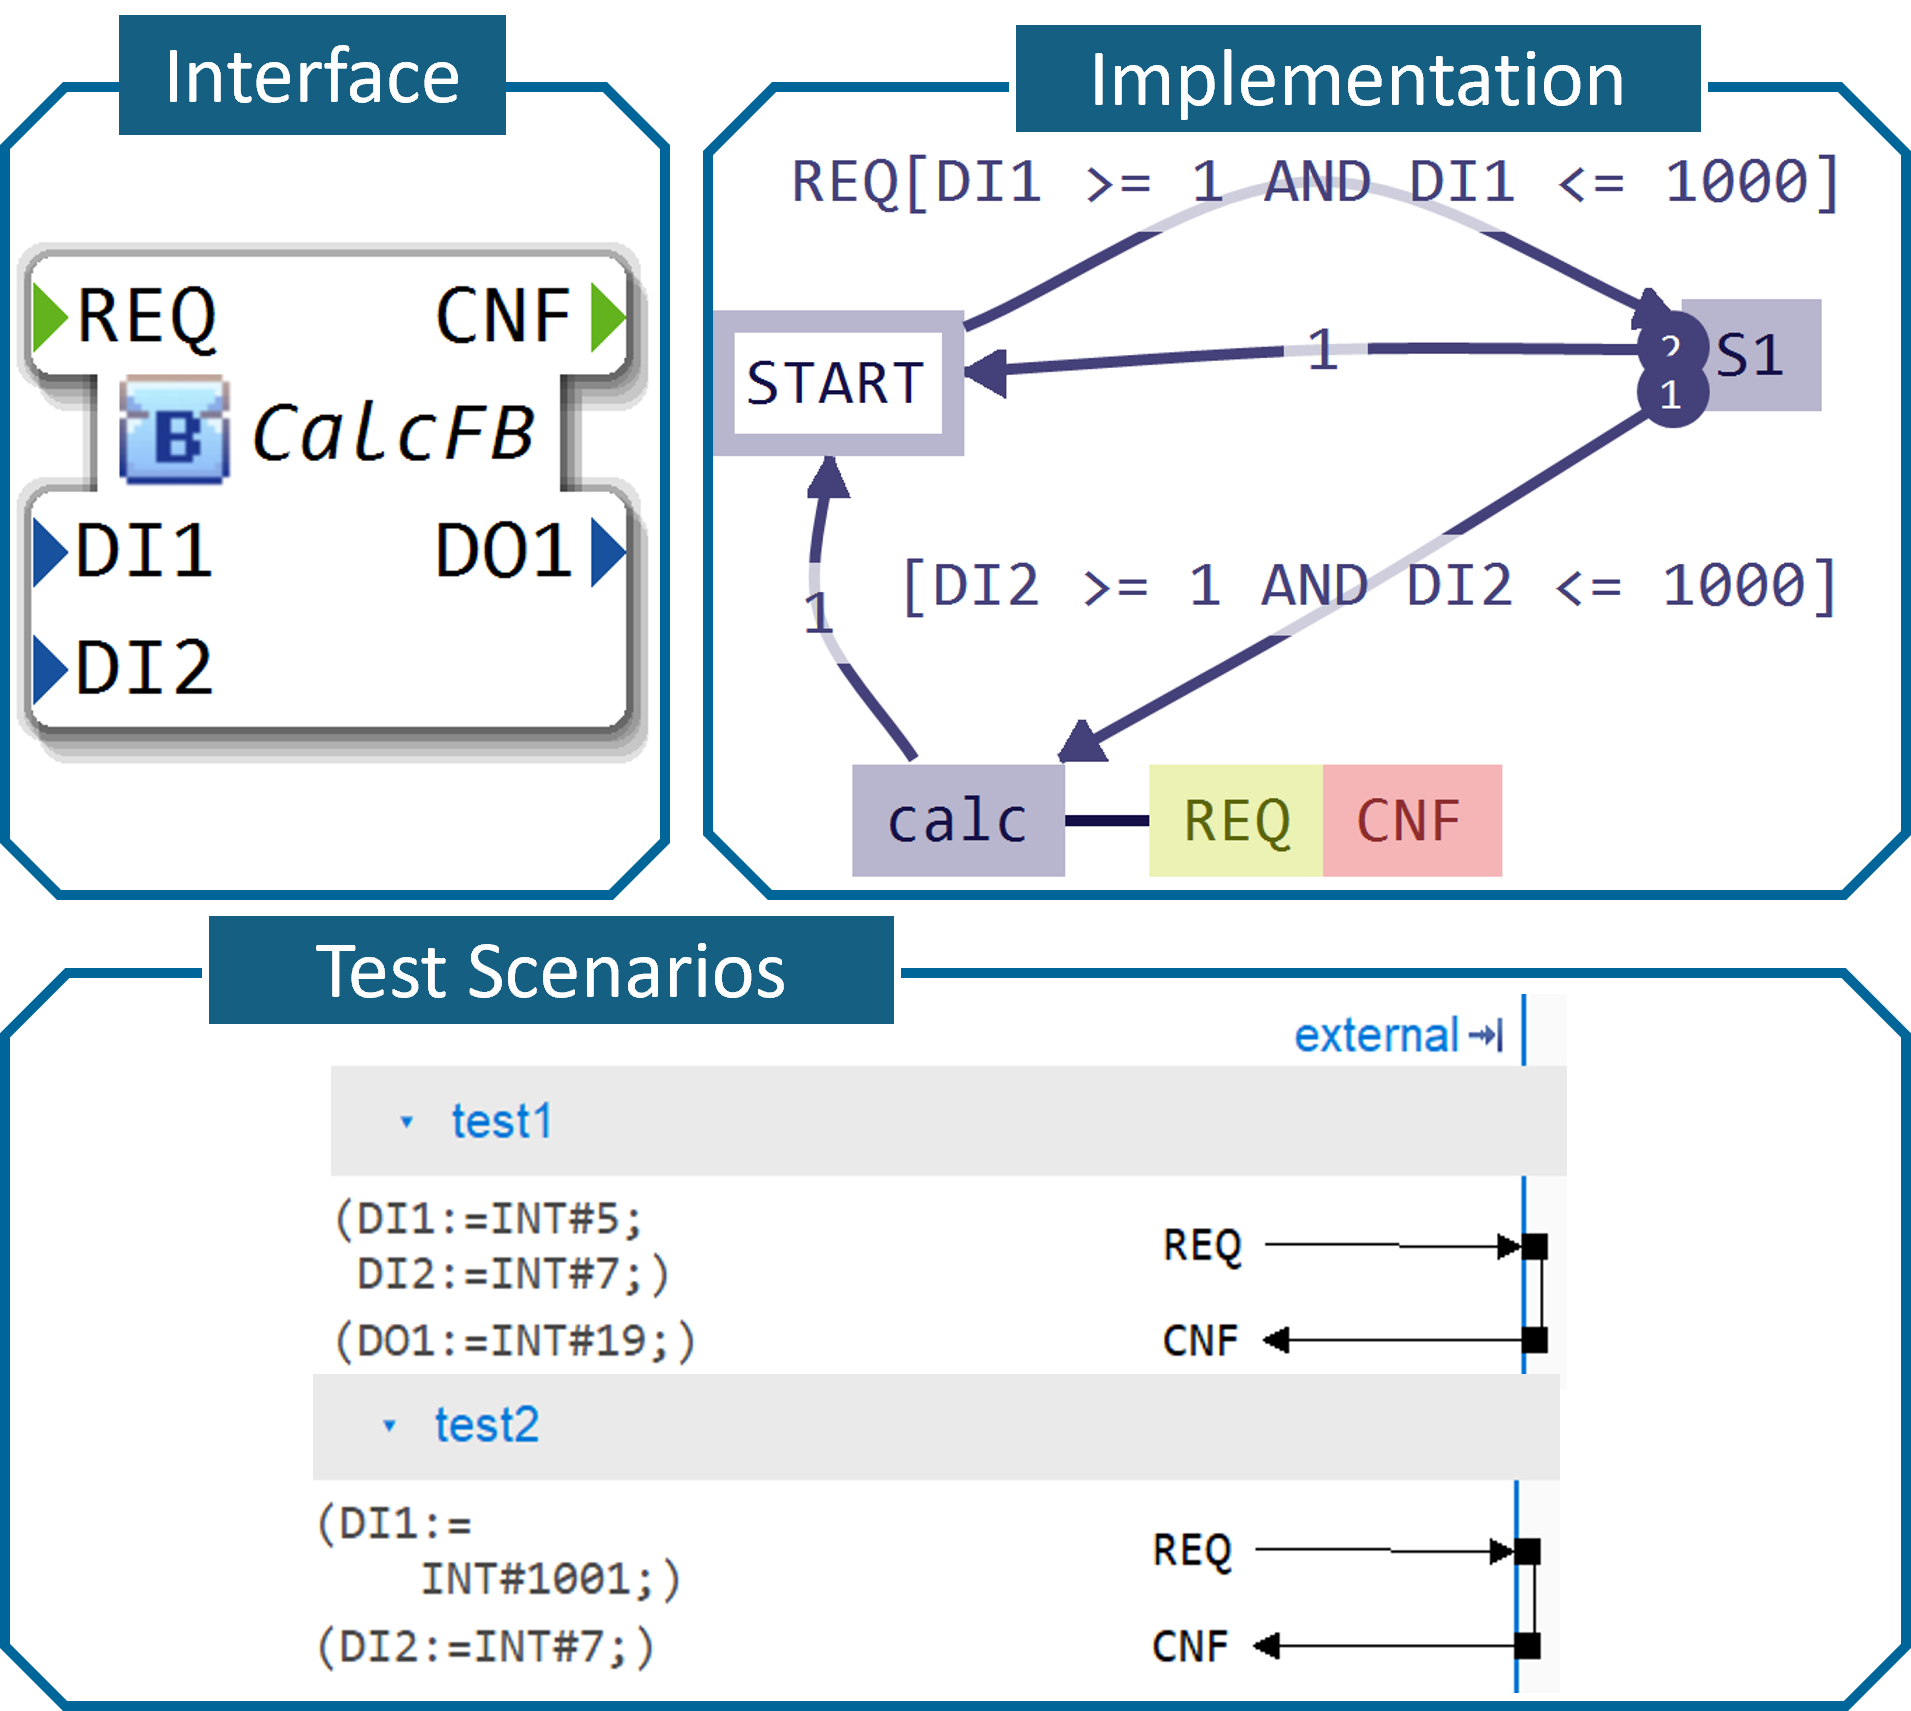
\includegraphics[width=0.75\columnwidth]{OJIES_2024/Figures/RunningExample.png}
    \caption{Running Example: FB performing simple calculation. FB interface defining the component, implementation as state diagram, and two usage scenarios modelled as service sequences.}
    \label{fig:running_example}
\end{figure}
\begin{figure*}[t!]
	\centering
	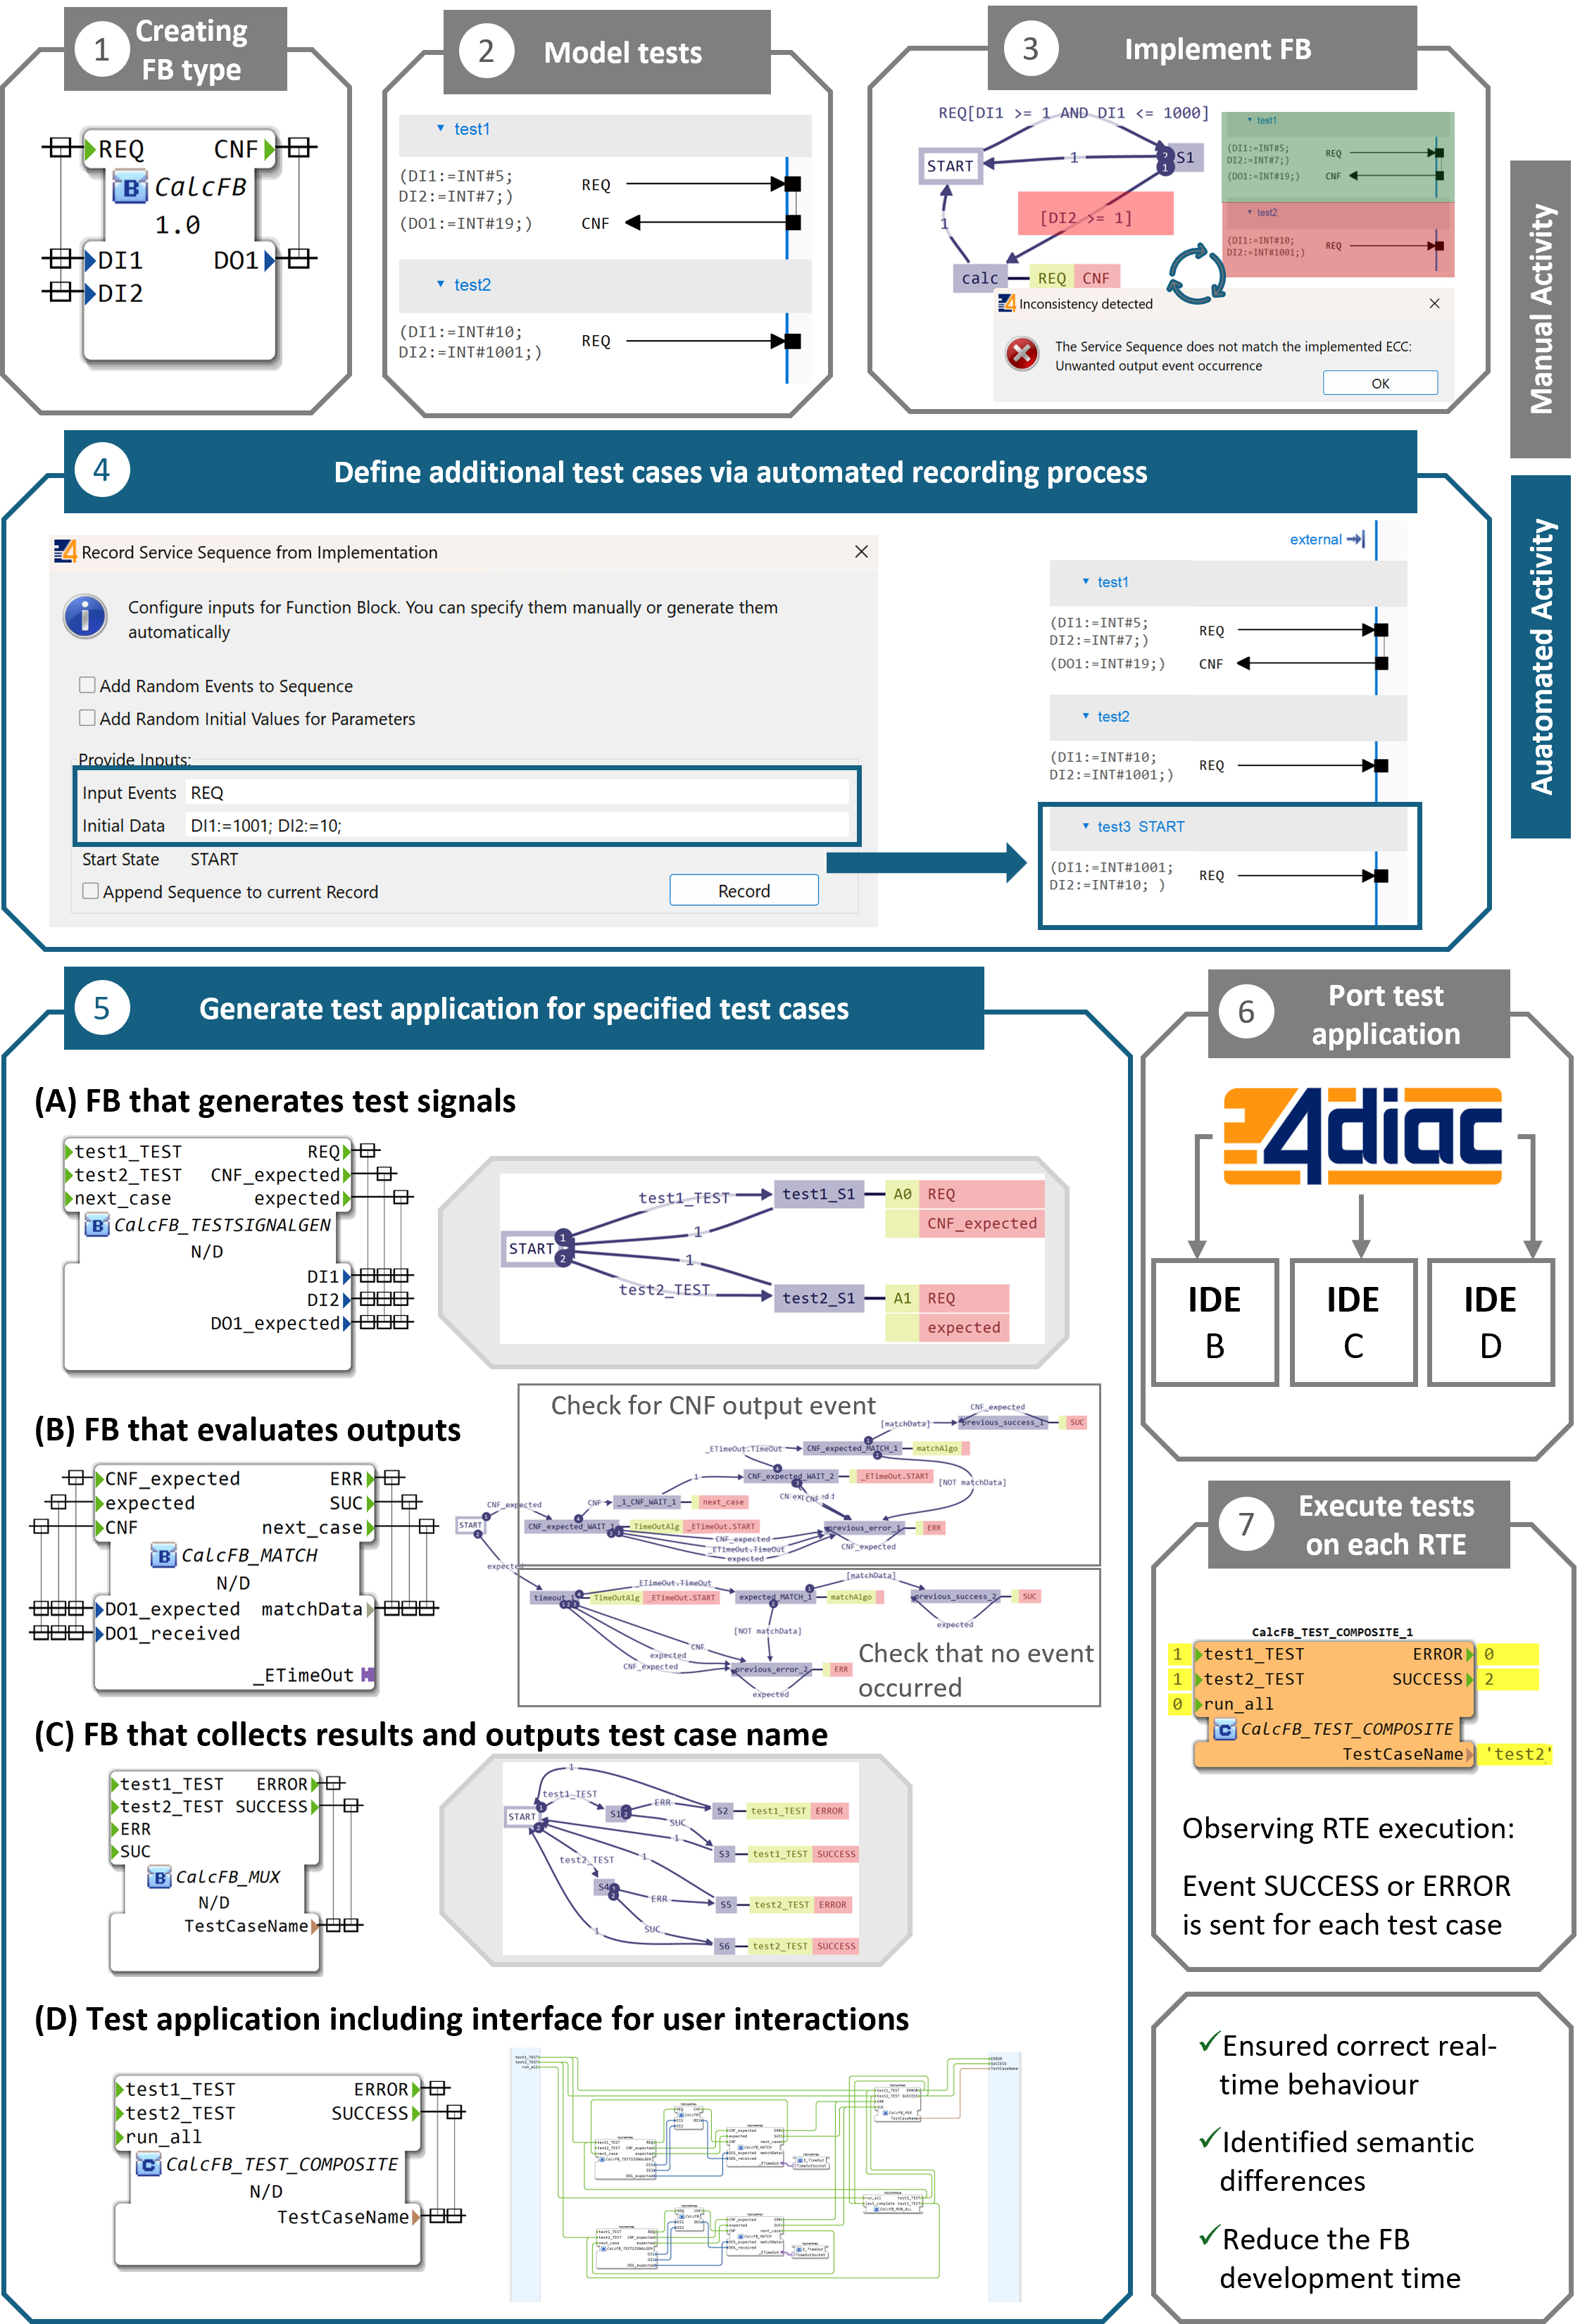
\includegraphics[width=0.85\textwidth]{OJIES_2024/Figures/methodology_complete.png}
	\caption{Overview of process for testing FBs across various software platforms. The seven-step process is partly automated with tools (blue boxes), partly it requires tool-assisted manual development. The test application can be ported to tools of various vendors and validate the expected behaviour of an FB directly in the target RTE, thus, possibly identifying differences in the execution semantics that affect the FB under test.}
	\label{fig::methodology}
\end{figure*}

\begin{itemize}
   \item Input event \texttt{REQ} triggers the calculation.
   \item Data inputs \texttt{DI1}, \texttt{DI2} receive values from other FBs and are used in the algorithm.
   \item The data output \texttt{DO1} stores the result of the algorithm.
   \item The output event \texttt{CNF} is issued to indicate that the algorithm was completed and that the output result is ready to be used by other FBs.
   \item The algorithm \texttt{REQ} within the FB is executed whenever the input event \texttt{REQ} occurs. The algorithm assigns the result of the formula to the output variable DO1.
%Once the algorithm execution is completed, the function block triggers the CNF event to indicate that the output result is ready to be used or transmitted to other function blocks.
\end{itemize}

In our example, the FB performs the calculation if the values of \texttt{DI1} and \texttt{DI2} are between 1 and 1000 (cf. implementation of the state diagram in Figure~\ref{fig:running_example}). When triggering the \texttt{REQ} event with appropriate input values, the FB executes the algorithm and produces the respective output. Both cases are modelled as service sequences and serve as test scenarios for the running example.
%\subsection{Running Example: Service Model}


\section{Methodology for Testing FBs}
\label{sec::methodology}
Our proposed approach for cross-platform FB testing is suitable for a test-driven development process, as well as for testing existing implementations. It involves specifying tests, executing tests within an IDE, generating the portable test application, as well as executing these tests on all relevant RTEs. A test application that is compliant with IEC~61499 can be ported to RTEs of various vendors. The approach is visualised in Figure~\ref{fig::methodology} as a step-by-step approach using the generated test cases of our running example (Section~\ref{sec::running_example}). In the following, we describe each step of the process in detail. We describe the envisioned development process based on our running example. %Detailed transformation rules for the generation of IEC~61499 software will be described in Section~\ref{sec::transformationrules}.

\subsection{Test-driven Development of FBs}
The following steps describe a test-driven development process. For testing existing FB libraries, the process starts directly at step 4, as the implementation is already complete. In this case, test cases will be generated semi-automatically from the implementation to reduce the effort.

\subsubsection{Creating a new Function Block type (FBT)}
Reusable functionality should be encapsulated in an FB. This involves specifying the input/output events and data inputs/outputs. %Unless the developer adheres to a test-driven development (TDD) process, the internal behaviour of the FB is implemented as well. 
For the running example, this involves defining the interface of the calculation FB.

\subsubsection{Specify test cases as service sequence models} Specification models are defined.
   %In this step, the test cases for the FB are specified as service models. There are two approaches to this:
   % \begin{enumerate}
   % \item Manually defining Service Sequences: The test cases are manually defined as service sequences, representing the expected behaviour of the FB under different scenarios.
  %  \item  Recording Service Sequences using the interpreter: Alternatively, the test cases can be recorded using the interpreter, which 
 %   \end{enumerate}
In the running example, a service model with two sequences is provided to define the test scenarios for the FB (cf. Figure~\ref{fig::methodology}, step 2). The service model specifies the expected event occurrences, as well as the input values (\texttt{DI1} and \texttt{DI2}) and the expected output value (\texttt{DO1}) for each test case.  
The scenario of \texttt{test1} is triggered upon arrival of an event at the input \texttt{REQ}. The purpose of \texttt{test1} is to describe the FB behaviour by checking whether it correctly returns 19 when given input values of 5 and 7. 
Additionally, \texttt{test2} aims to evaluate the FB behaviour for an edge case, as one value will be out of range (i.e., \texttt{DI2:=INT\#1001}). We expect that no addition is performed, and no output events are sent (cf. second sequence in step 2). 
Where output data values are expected, they are specified together with the output event. %it can be determined whether the FB behaves as intended.
% TODO BIANCA adds the figures to this sequence

    \subsubsection{Implement desired functionality of the FB type}
    When following a TDD process, the functionality of the FB is implemented at this stage. The specified tests can be used for iteratively evaluating the correctness. For instance, the implemented behavior of an FB can be analysed using model interpreters to receive rapid feedback on any changes. 
    For the running example, we assume that the limit check of DI2 was not yet implemented. This scenario is illustrated in step 3 of Figure~\ref{fig::methodology}. When the test cases are executed using a model interpreter \cite{wiesmayr2021}, the feedback shows that an unexpected event occurrence (i.e., CNF) has been output by the FB under test. 
    By comparing the actual output with the expected output for each test case, the implemented FB behaviour is evaluated automatically.
    As a result, the transition condition of the state diagram can be updated to include the missing check for \texttt{DI2<=1000}. Afterwards, evaluating the service sequence is successful.

\subsection{Testing Implemented FBs}
    After an FB has been developed, it needs to be evaluated in an RTE. While manual testing is feasible on all existing RTEs, automating the process allows to reduce the development time and effort. Hence, the following steps describe the process of model-based testing by generating an IEC~61499-based test application from the test specification.

\setcounter{subsubsection}{3}
   \subsubsection{Defining (additional) test cases for the implemented FB}
    Especially when validating the behavior of an FB in different platforms, creating test cases for additional corner cases may be useful. Even when a test-driven development approach is followed, a comprehensive test suite may not be available. Using a model interpreter and its accompanying execution framework~\cite{wiesmayr2021} allows recording additional test cases based on specified events and/or data inputs. This also allows adding test suites to existing implementations.  Step 4 in Figure~\ref{fig::methodology} shows the dialogue for recording a service sequence where DI1 is out of range. The resulting graphical diagram is added to the FB type specification and is shown on the right. Developers have to manually check whether the result matches the expected behaviour of the developed FB. Recorded tests can serve as regression tests, as they capture the actual behaviour of an executed FB. This can ensure that an FB is evaluated comprehensively during model evolution. 
  
\subsubsection{Generate test application for specified test cases}
    Once the implementation has been completed, the correct real-time behavior of an FB has to be evaluated in a run-time environment. The test application ensures that developers do not need to manually interact with an FB and observe the outputs. Hence, various components are required for issuing test signals, which can be automatically generated. They are visualized in step 5 of Figure~\ref{fig::methodology} and described as follows:
    \begin{itemize}
        \item \textbf{(A) Test signal generator:} This FB generates the input signals based on the service model and supplies the required events and data to the FB under test (REQ, DI1, DI2). It also notifies the test application of the expected output events (CNF or none). Additionally, it provides the expected output values (DO1), which are set in algorithms. 
        \item \textbf{(B) Matcher:} This FB compares the execution results of the FB under test with the expected results that are provided by the test signal generator. 
        \item \textbf{(C) Multiplexer: } The next FB forwards the result (ERROR, SUCCESS) of each test case (i.e., service sequence) to the output, together with the name of the executed test case. This helps developers to identify the faulty test case if there are any problems. 
        \item \textbf{(D) Test application composite: } A composite FB encapsulate the test application so that it can be easily deployed to an RTE. All components are interconnected to provide a simple interface. Developers can run each test case by triggering the respective events. An additional event pin ``run\_all'' is provided to execute all test cases sequentially based on a single event trigger. This functionality is handled by an additional FB which initiates these further test cases. 

    \end{itemize}
        Some of the components (e.g., the matcher) also require a timer to wait for the results of the FB under test, thus, ensuring that no unexpected event outputs are detected. As a result, timer FBs are included in the test application.
        Note that the test signal generator, the FB under test, and the matcher are instantiated once per test case. This ensures that the internal state of these components does not affect further test cases. The FBs are guaranteed to initiate the execution from the START-state. As all FBs for the test application require an internal state, they are realized as Basic FBs. Although Figure~\ref{fig::methodology} visualizes the test environment for a Basic FB (i.e., the running example), any kind of FB can serve as the FB under test. Only the interface definition and the service model are required. This also means that application parts can be tested as long as they are integrated into an FB.

Based on the results provided in \cite{Testing_Midhun,biancaMidhunETFAwip}, we derived transformation rules for creating test code from service models. We implemented these rules in Eclipse 4diac~\cite{eclipse4diac}, which provides an open source IDE for IEC 61499-based software.
\begin{figure*}
    \centering
    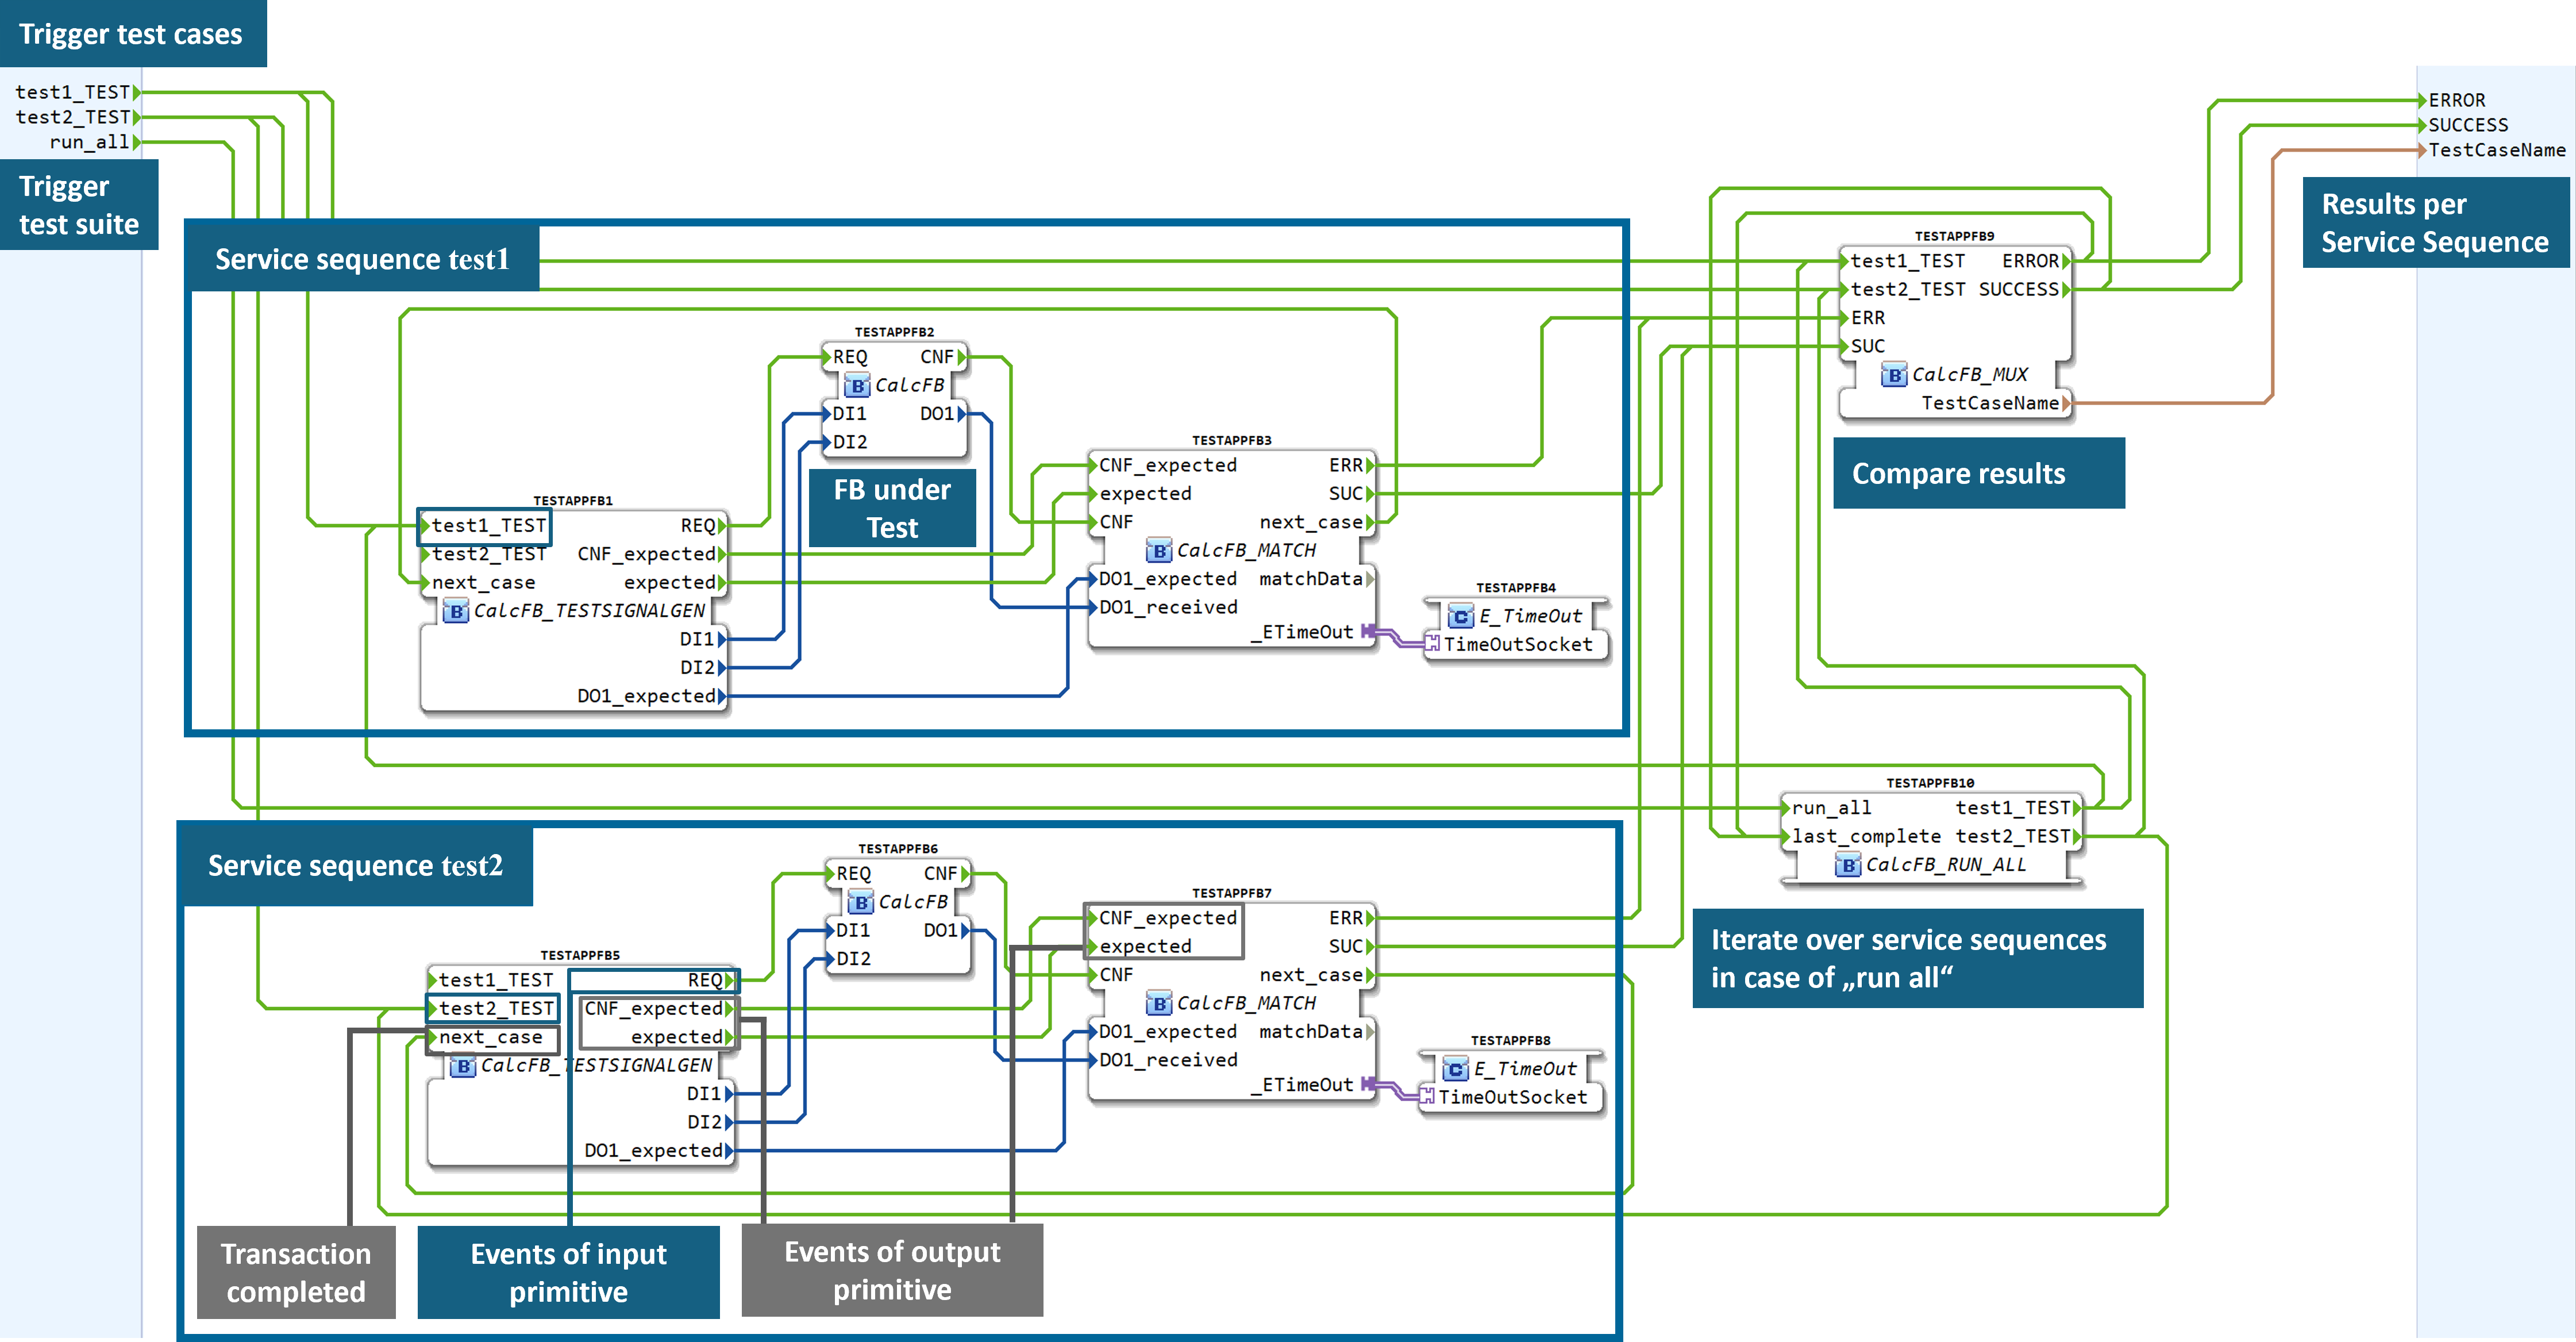
\includegraphics[width=\linewidth]{OJIES_2024/Figures/generation_rules.png}
    \caption{Test application generated for two service sequences of the running example. Relevant regions are highlighted including their relation to the service model.}
    \label{fig::testapp}
\end{figure*}

\begin{itemize}
        \item  A \textbf{service model} serves as the test suite and includes one or more service sequences. A single test application is generated for the whole service model. 
        
        \item Each \textbf{service sequence} serves as one test case. We need one event input per test case in the test application FB, which will trigger the execution of this test. We include its name in the event pin to relate the parts of the test application with the respective service sequences. Once the service sequence was completed, an ERROR or SUCCESS event is issued, together with the name of the service sequence. A service sequence can consist of several service transactions, which define the flow of events along the sequence. 
         
         \item Each \textbf{service transaction} is comprised of an input primitive (ingoing arrow) and any number of output primitives (outgoing arrows). The service transactions are processed one after another. An event issued by the matcher (nextCase) indicates that a transaction has been completed.
        
        \item The \textbf{input primitive} describes the event that initiates a transaction. 
        The test signal generator FB has to issue the input event specified in a transaction. They are supplied to the FB under test via the respective connections together with the associated data. As a result, the test signal generator FB requires one output pin (events and data) for each input pin of the FB under test. 
        
        \item The \textbf{output primitives} describe the event(s) that is/are caused by the input event.
        The test signal generator FB issues an event indicating all output events that are part of a test sequence. They are supplied to the FB under test via the respective connections together with the associated data. As a result, the test signal generator FB requires one output pin (events and data) for each input pin of the FB under test. The matcher FB receives information about the expected events and data values from the signal generator FB. It compares them with the events and data received from the FB under test.
\end{itemize}


\subsubsection{Port test application to other platforms}
The presented development approach is fully supported in 4diac~IDE~\cite{eclipse4diac}. Although service sequences are defined in the standard, they are not fully supported in other tools. Also the model execution framework for evaluating FBs is provided in 4diac~IDE. Hence, the test application is generated in 4diac~IDE following the notation of the IEC~61499 standard, and is then ported to other platforms. Manual effort may be required for importing FBs developed in one IDE to other vendors \cite{cheng_pang_portability}.

\subsubsection{Execute Tests in All Relevant RTEs}
The generated test application (i.e., the composite FB), is deployed to and executed on different RTEs. The behaviour and output results of the FB are evaluated manually in each RTE.




\section{Implementation}
\label{sec::implementation}
Sophisticated tool support can automate a large part of the process, especially for the steps 4 to 6. The systematic approach ensures that FBs can be thoroughly tested for functionality and compatibility across various RTEs.
Tool support for specifying service sequences and simulating their results is available in 4diac IDE from previous work \cite{wiesmayr2021}. We have extended the tool with a test FB generator, which uses the information provided in service models to create test code. Unlike the prototype presented in \cite{biancaMidhunETFAwip}, the current implementation fully automates the process of creating control code and supports all kinds of test cases that can be modeled in service sequences. The code is available open source on Github.\footnote{\url{https://github.com/eclipse-4diac/4diac-ide/tree/release/plugins/org.eclipse.fordiac.ide.fb.interpreter}}


\subsection{Case Study: Processing Station}
\label{sec::casestudy}
\label{sec:drilling}
 
The processing station (Figure~\ref{fig:ps}) is composed of several mechatronic components, including the table, tester,  and drill component. They are considered smart, i.e., each is equipped with its own control devices, implementing the provided operations. The table component undergoes rotation from one fixed position to another. A complete cycle is achieved when the table rotates six times. Whenever a material is positioned in the loading area, the table rotates to align it underneath the tester component. The tester then checks whether the material has been drilled. If necessary, the drill component is triggered to process the material as soon as its sensor detects it. 

\begin{figure}[!t]
	\centering
		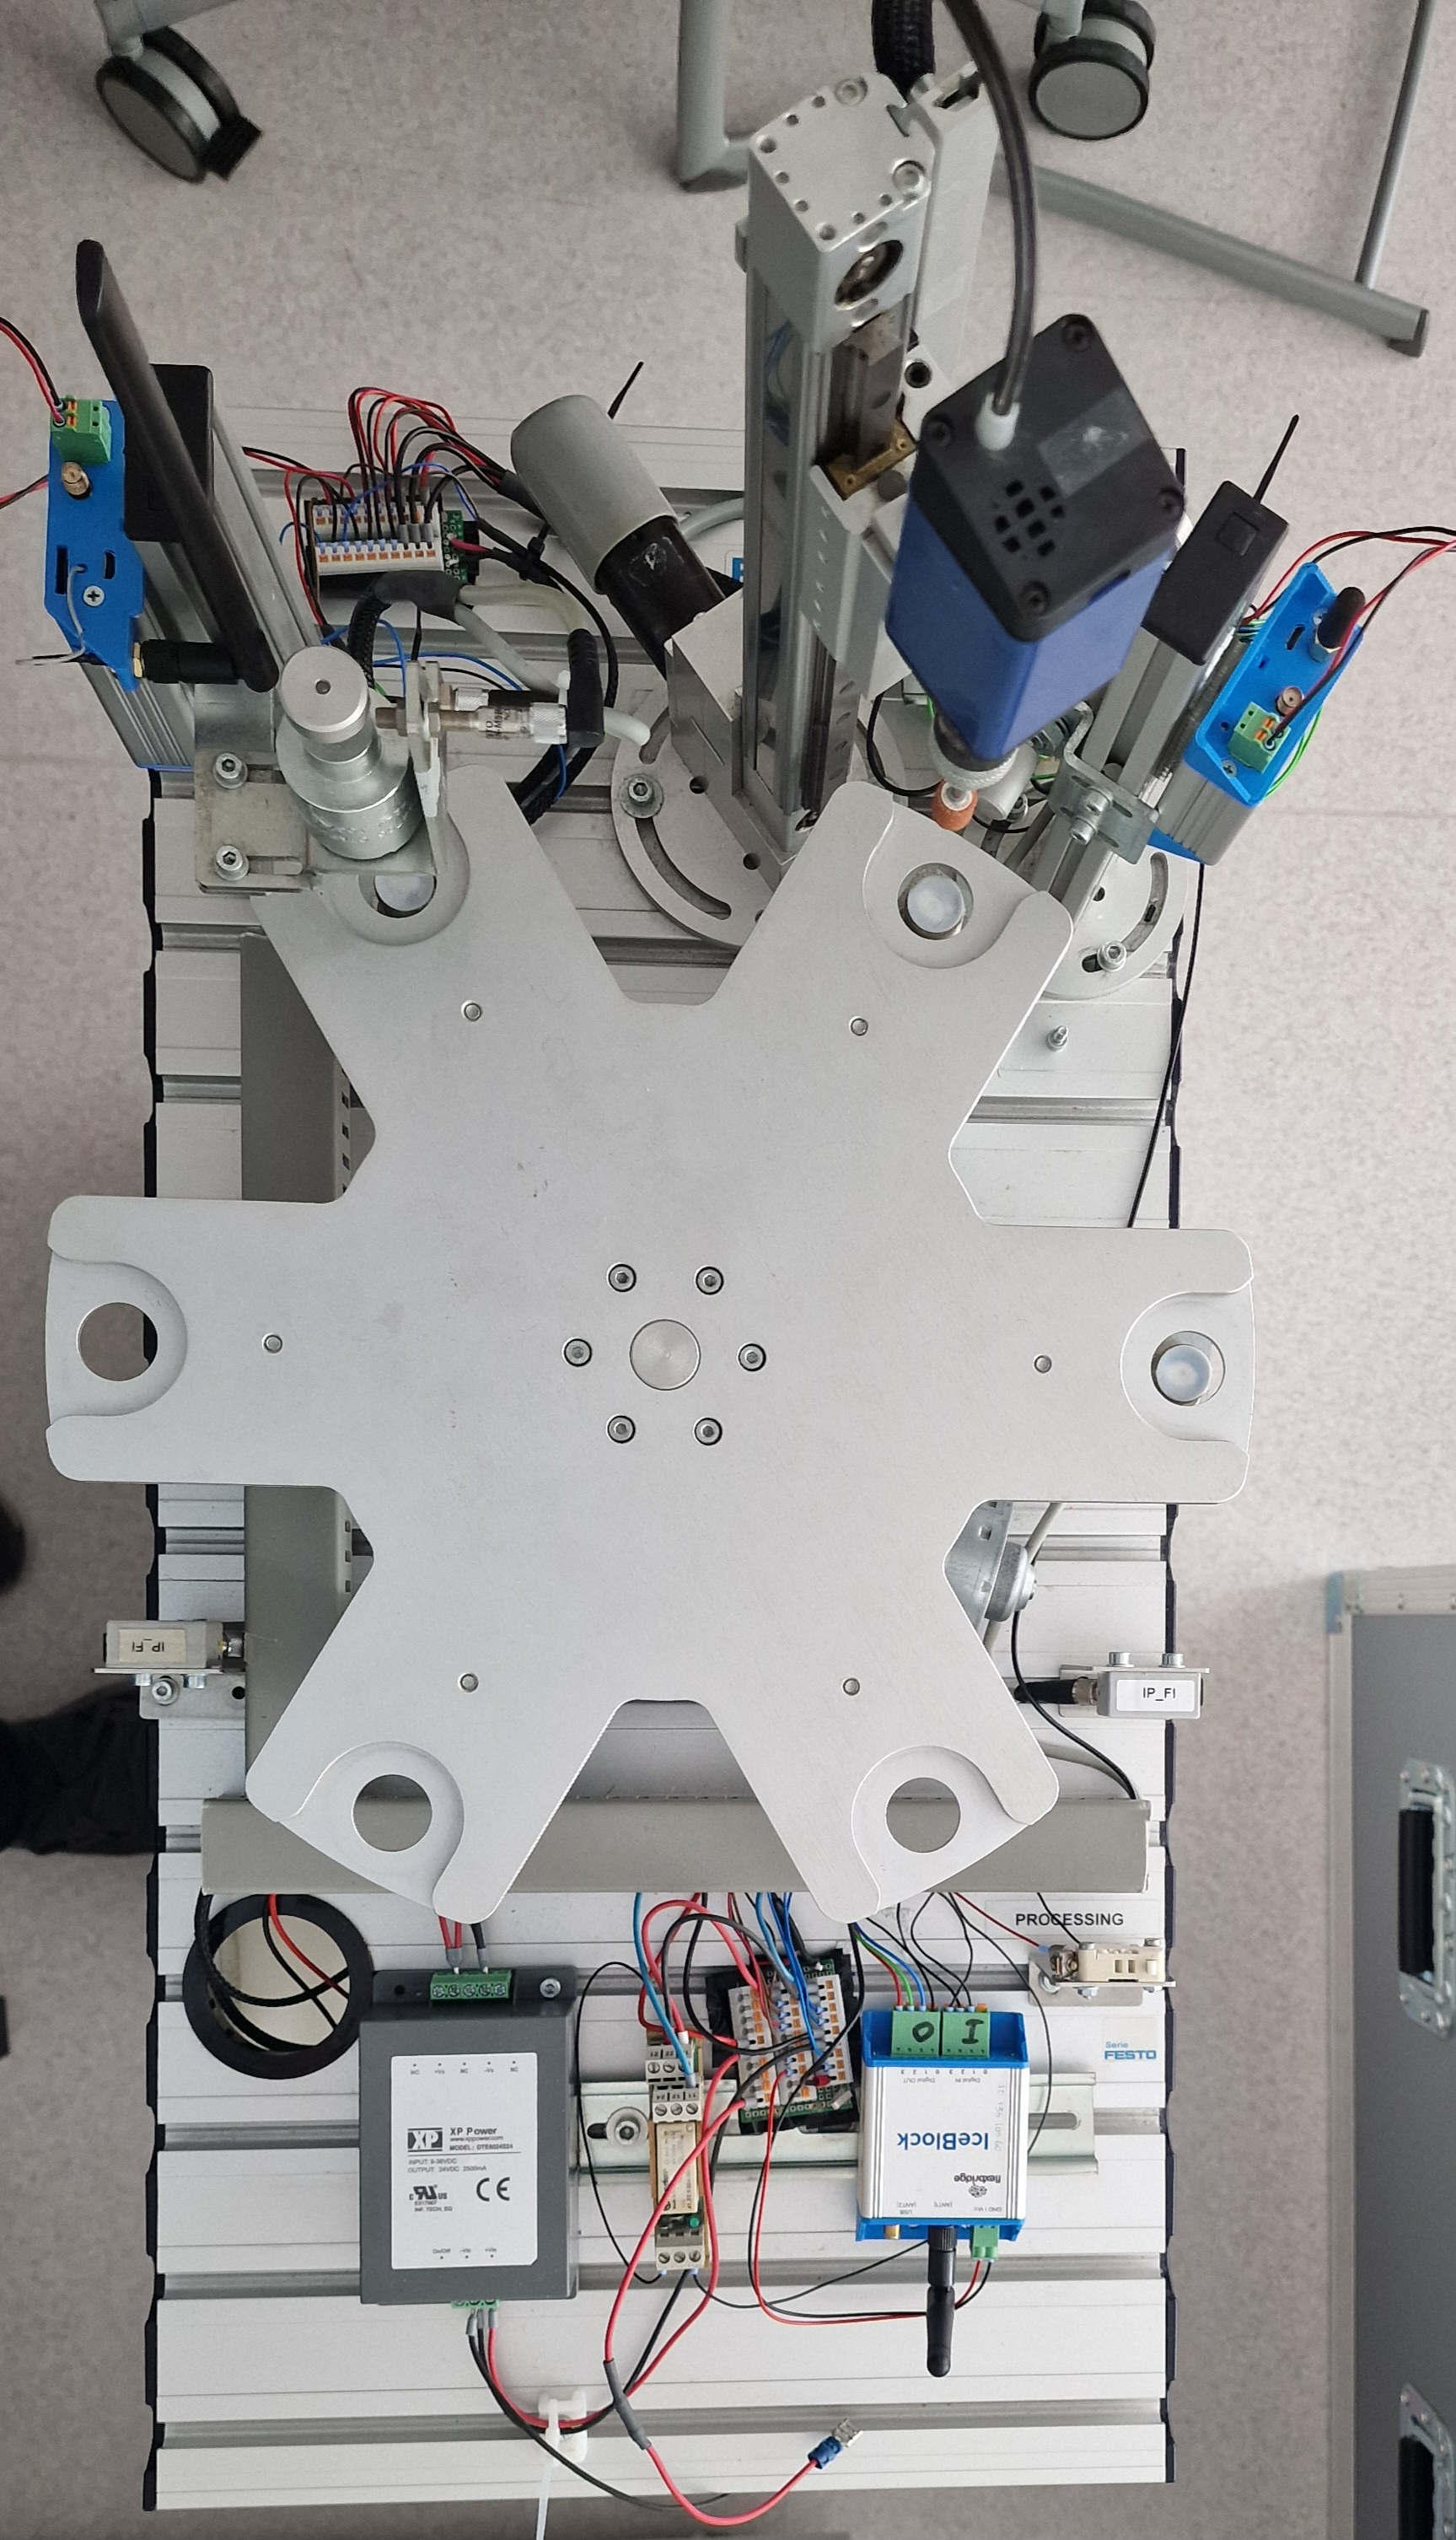
\includegraphics[width=0.5\linewidth,clip]{OJIES_2024/Figures/processingStation.jpg}
		\caption{Processing station}
		\label{fig:ps}	
 \end{figure}

The processing station system implemented in IEC~61499 is designed to control various mechatronic components through an integrated application. Each of these components is equipped with its own control device, which execute distinct control programs, i.e., the TableControl, TesterControl, and DrillControl programs. The application is implemented following the "Chain of Actions" design pattern \cite{Patil.2018}, which draws inspiration from the "Chain of Responsibility" design pattern. Each of the components is implemented as a FB network that is shown in Figure~\ref{fig:Application}. For the evaluation, three Basic FBs controlling the respective substations will be presented in detail.

\subsubsection{Table Control: Rotation}
The TableControl FB network (cf. Figure~\ref{fig:Application} \textit{top}) is responsible for rotating the table to position the material appropriately under the tester and drill components. The \texttt{WPdeliveryService} FB, a composite FB encapsulating another FB network, manages this rotation through the \texttt{TableDriver} FB and a pair of \texttt{E\_DELAY} FBs. The latter are part of the core FB library defined in the standard. Multiple instances of \texttt{WPdeliveryService} are included in the control application. 

The \texttt{TableRotate} FB encapsulates the core control logic within the network, making it the primary focus for testing the component's features. Its interface and state diagram are shown in Figure~\ref{fig:TableRotate}. The FB controls the rotational movement of a table machine which can rotate to different positions as required by the system's operation through state transitions. The primary functions include starting the rotation, monitoring the rotation process, checking if the table is in the correct position, and handling timeouts. This FB ensures that the table's motion is accurately controlled and stops when the desired position is reached or if a timeout occurs. As shown in the FB interface, the main events are \texttt{ROTATE} and \texttt{TIMEOUT\_EXCEED}. The \texttt{inPosition} input variable signals that the table has reached its target position, while output events such as \texttt{DRIVE\_ON}, \texttt{DRIVE\_OFF}, and \texttt{DONE} manage the rotation process. The state diagram (i.e., ECC) initially has an active \texttt{START} state, moves to \texttt{ROTATE\_START} when the rotation begins, and transitions to \texttt{ROTATE\_CONTINUE} if a timeout occurs. Once the table is in position, the FB transitions to \texttt{DONE}, stops the rotation, and then returns to \texttt{START}, ensuring precise control of the table's movement. Two test scenarios for the timeout are included as service sequences in Figure~\ref{fig:TableRotate}. They show that the drive is switched off if the position has been reached. The scenarios ensure that the rotation is stopped even if the signal \texttt{inPosition} is not received correctly. 
%\todo[inline]{MX: please check that the sequences (test cases) seem correct.}
\begin{figure}[bt]
	\centering
		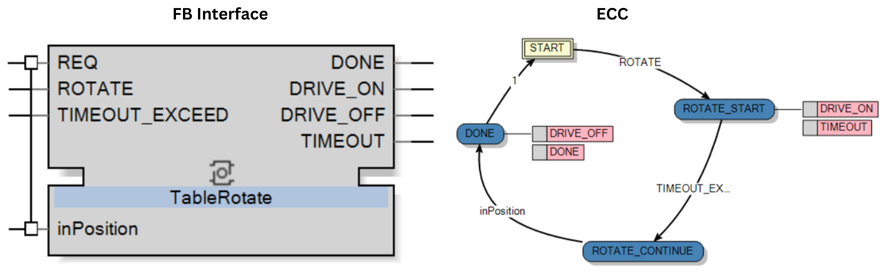
\includegraphics[width=0.99\linewidth,clip]{OJIES_2024/Figures/TableRotate.png}
            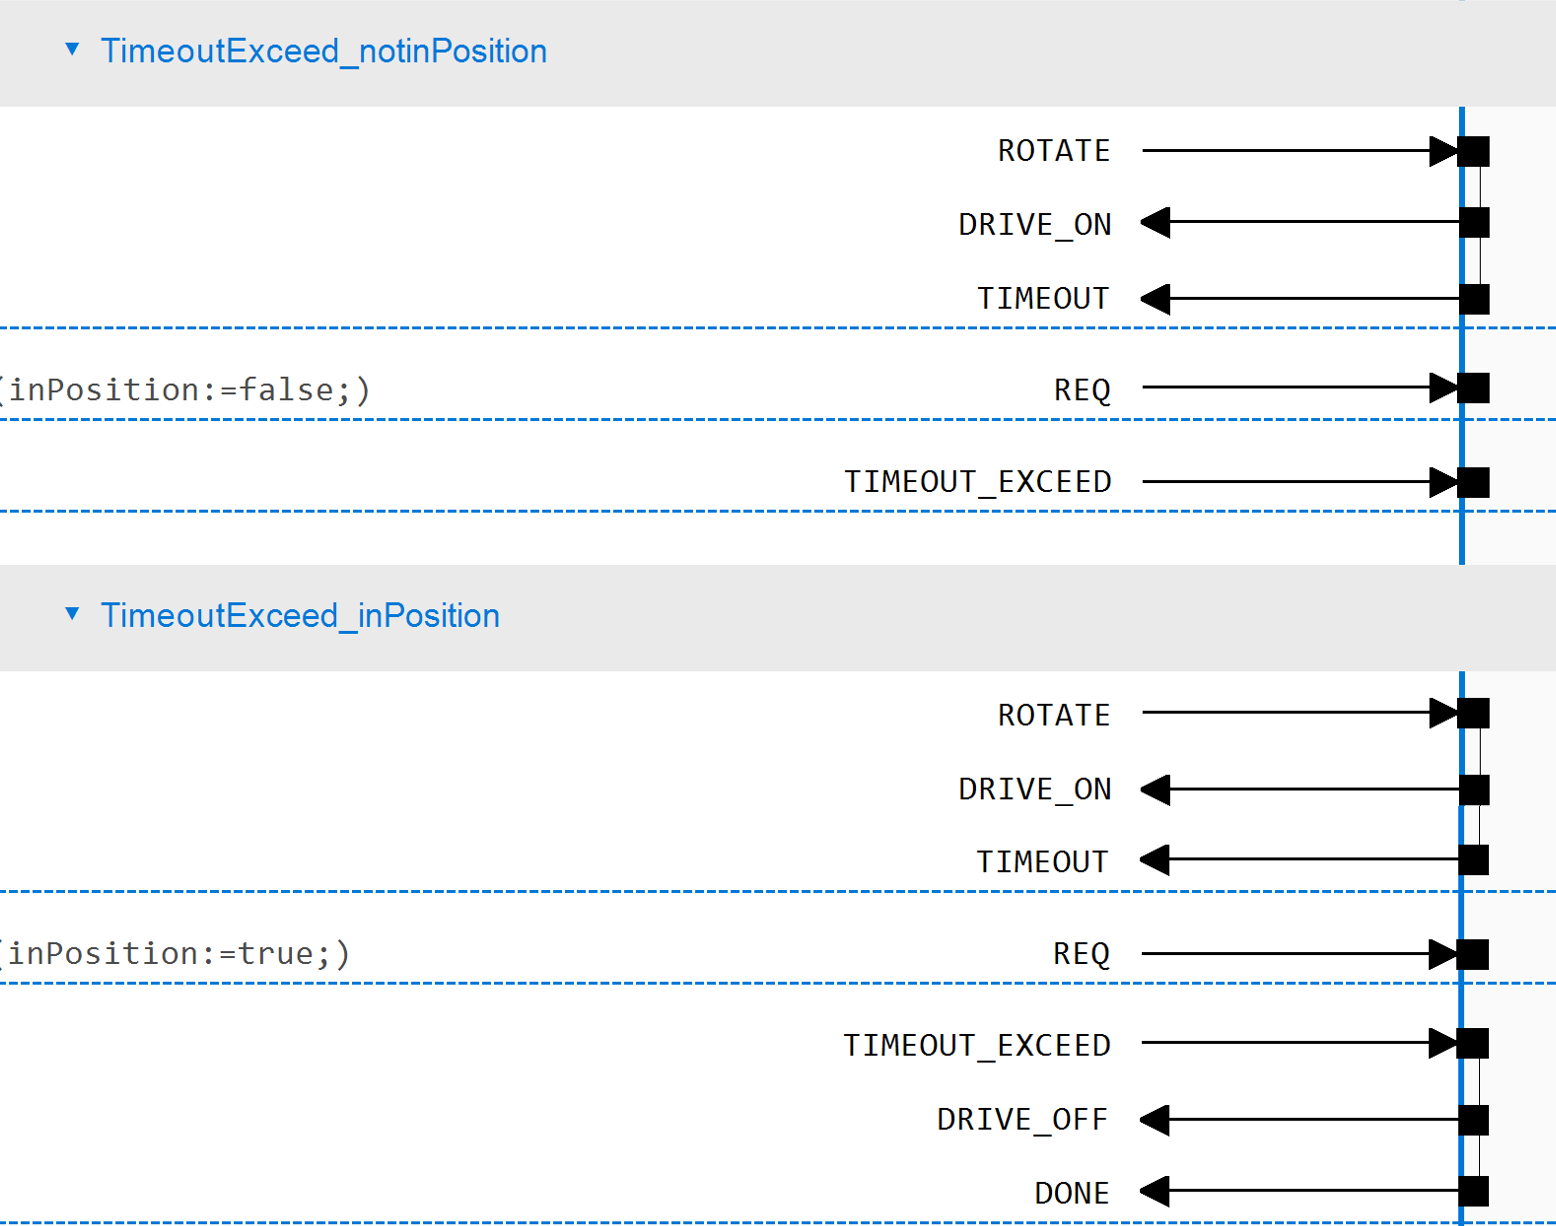
\includegraphics[width=0.99\linewidth]{OJIES_2024/Figures/tests_casestudy/Service-TableRotate_selected.png}
        \caption{TableRotate: Interface, state diagram, and selected test cases.}
		\label{fig:TableRotate}	
 \end{figure}
 \begin{figure*}[bt]
	\centering
		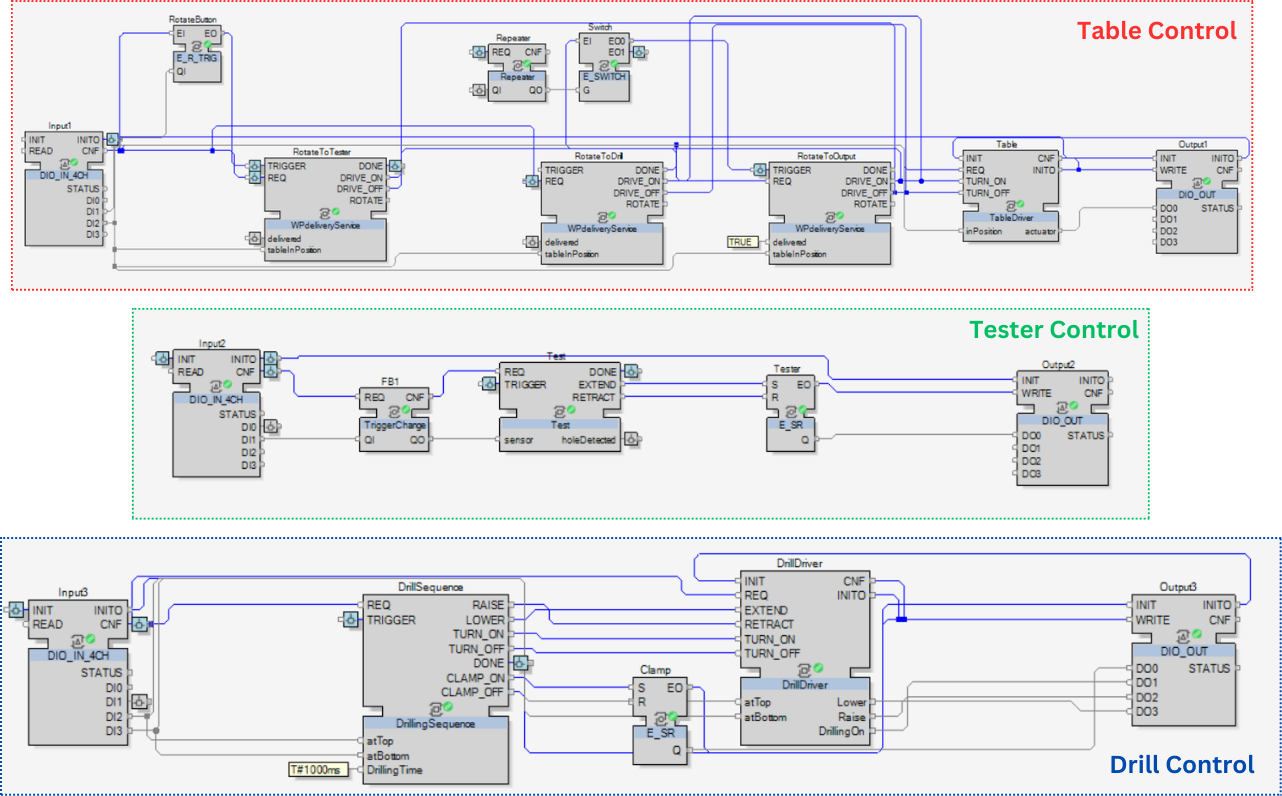
\includegraphics[width=0.99\linewidth,clip]{OJIES_2024/Figures/FB_App.png}
		\caption{Control applications for the three substations including input FBs for processing signals from the physical system, control blocks orchestrating the station, and output FBs for writing information to actuators.}
		\label{fig:Application}	
 \end{figure*}

\subsubsection{Tester Control: Inspection}
The FB network for the Tester component, TesterControl, detects holes in the workpiece to prevent that a workpiece is drilled more than once and to verify that the workpiece has undergone drilling. The main component is the Composite FB \texttt{Test} which is comprised of a standard library FB (\texttt{E\_DELAY}) and the \texttt{TestCtrl} Basic FB. 

Upon activation, the \texttt{TestCtrl} FB uses sensor data to check whether a hole is present in the workpiece. In this case, it confirms that drilling was complete. The FB manages the sequence of extending, checking, and retracting the probe, and handles timeouts in case the process takes too long. The interface and ECC of the FB are shown in Figure~\ref{fig:TestCtrl}. 
The primary input event, \texttt{TRIGGER}, initiates the detection sequence, with \texttt{QI} qualifying this event and \texttt{QO} reflecting the detection result. The FB has four output events: \texttt{EXTEND} to extend the sensor, \texttt{RETRACT} to retract it, \texttt{DONE} to signal that the process was completed, and \texttt{TIMEOUT} to initiate a timer. The ECC transitions from \texttt{START} to \texttt{EXTEND} upon receiving \texttt{TRIGGER}, and if a timeout occurs, moves to \texttt{CHECK} to determine whether a hole was detected. It then transitions to \texttt{RETRACT} and finally to \texttt{DONE}. A test case that shows the behaviour in the case of a timeout is shown in Figure~\ref{fig:TestCtrl}. 
\begin{figure}[h!]
	\centering
		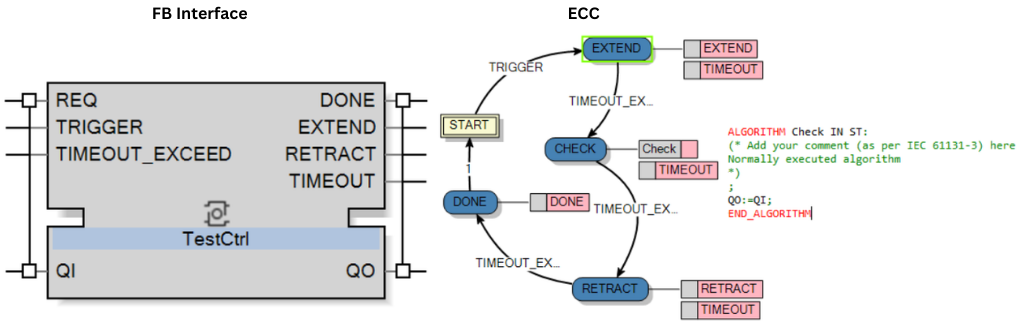
\includegraphics[width=0.99\linewidth,clip]{OJIES_2024/Figures/TestCtrl.png}
            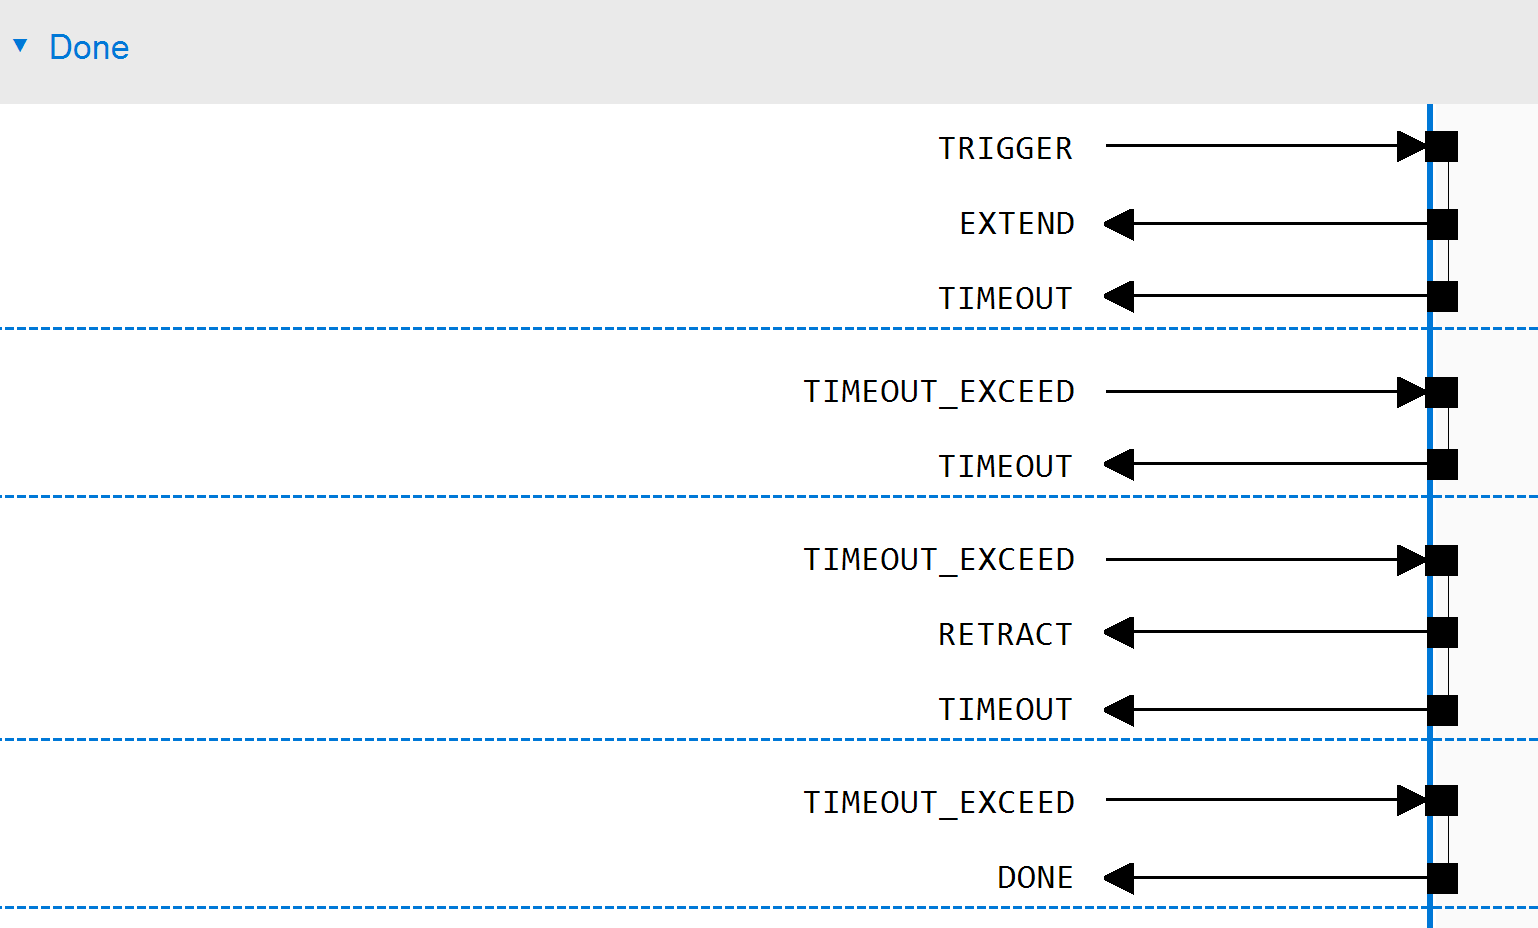
\includegraphics[width=0.99\linewidth]{OJIES_2024/Figures/tests_casestudy/Service-TestCtrl_timeout.png}
		\caption{TestCtrl: Interface, state diagram and a selected test case.}
		\label{fig:TestCtrl}	
 \end{figure}
 
\subsubsection{Drill Control: Processing}
The FB network for the drill component, DrillControl, orchestrates the drilling process. The main FBs are \texttt{DrillingSequence} and \texttt{DrillDriver}. The \texttt{DrillingSequence} is a composite FB that uses two FBs, \texttt{DoubleActingCylinder} and \texttt{SingleActingAc\-tu\-a\-tor}. The former is responsible for controlling the vertical movement of the drill, while the latter controls the rotation of the drill motor. As the \texttt{DoubleActingCylinder} FB contains the core logic of the drilling process, it is shown in Figure~\ref{fig:DoubleActingCylinder}. It controls the bidirectional motion of a drill machine, specifically managing its upward and downward movements. This control is essential for operating machinery that uses linear actuators, such as hydraulic or pneumatic cylinders, to extend and retract, corresponding to the downstroke and upstroke of the drill. The FB handles initialization, execution requests, extension (downward movement), and retraction (upward movement), with input conditions determining the cylinder's state transitions and output commands controlling the actuators.
Specifically, the cylinder movement is controlled via the events \texttt{EXTEND} and \texttt{RETRACT}. The input variables \texttt{atHome} and \texttt{atEnd} indicate the cylinder's position, while the output variables \texttt{extend} and \texttt{retract} command its motion. The ECC %manages transitions between states (\texttt{HOME}, \texttt{EXTEND}, \texttt{END}, and \texttt{RETRACT}), 
ensures that the cylinder moves correctly based on events and position feedback. The algorithms activate or stop the cylinder's movement, ensuring precise control for upward and downward motion. 
\begin{figure}[hbt]
	\centering
		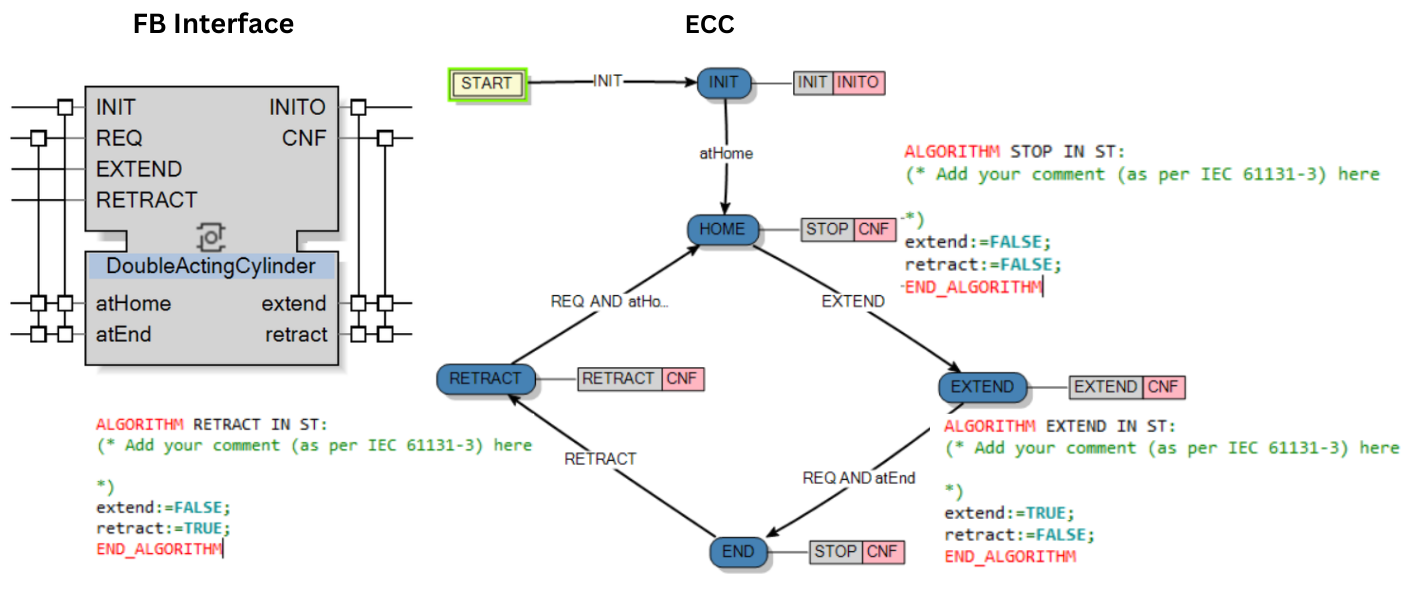
\includegraphics[width=0.99\linewidth,clip]{OJIES_2024/Figures/DoubleActingCylinderV2.png}
            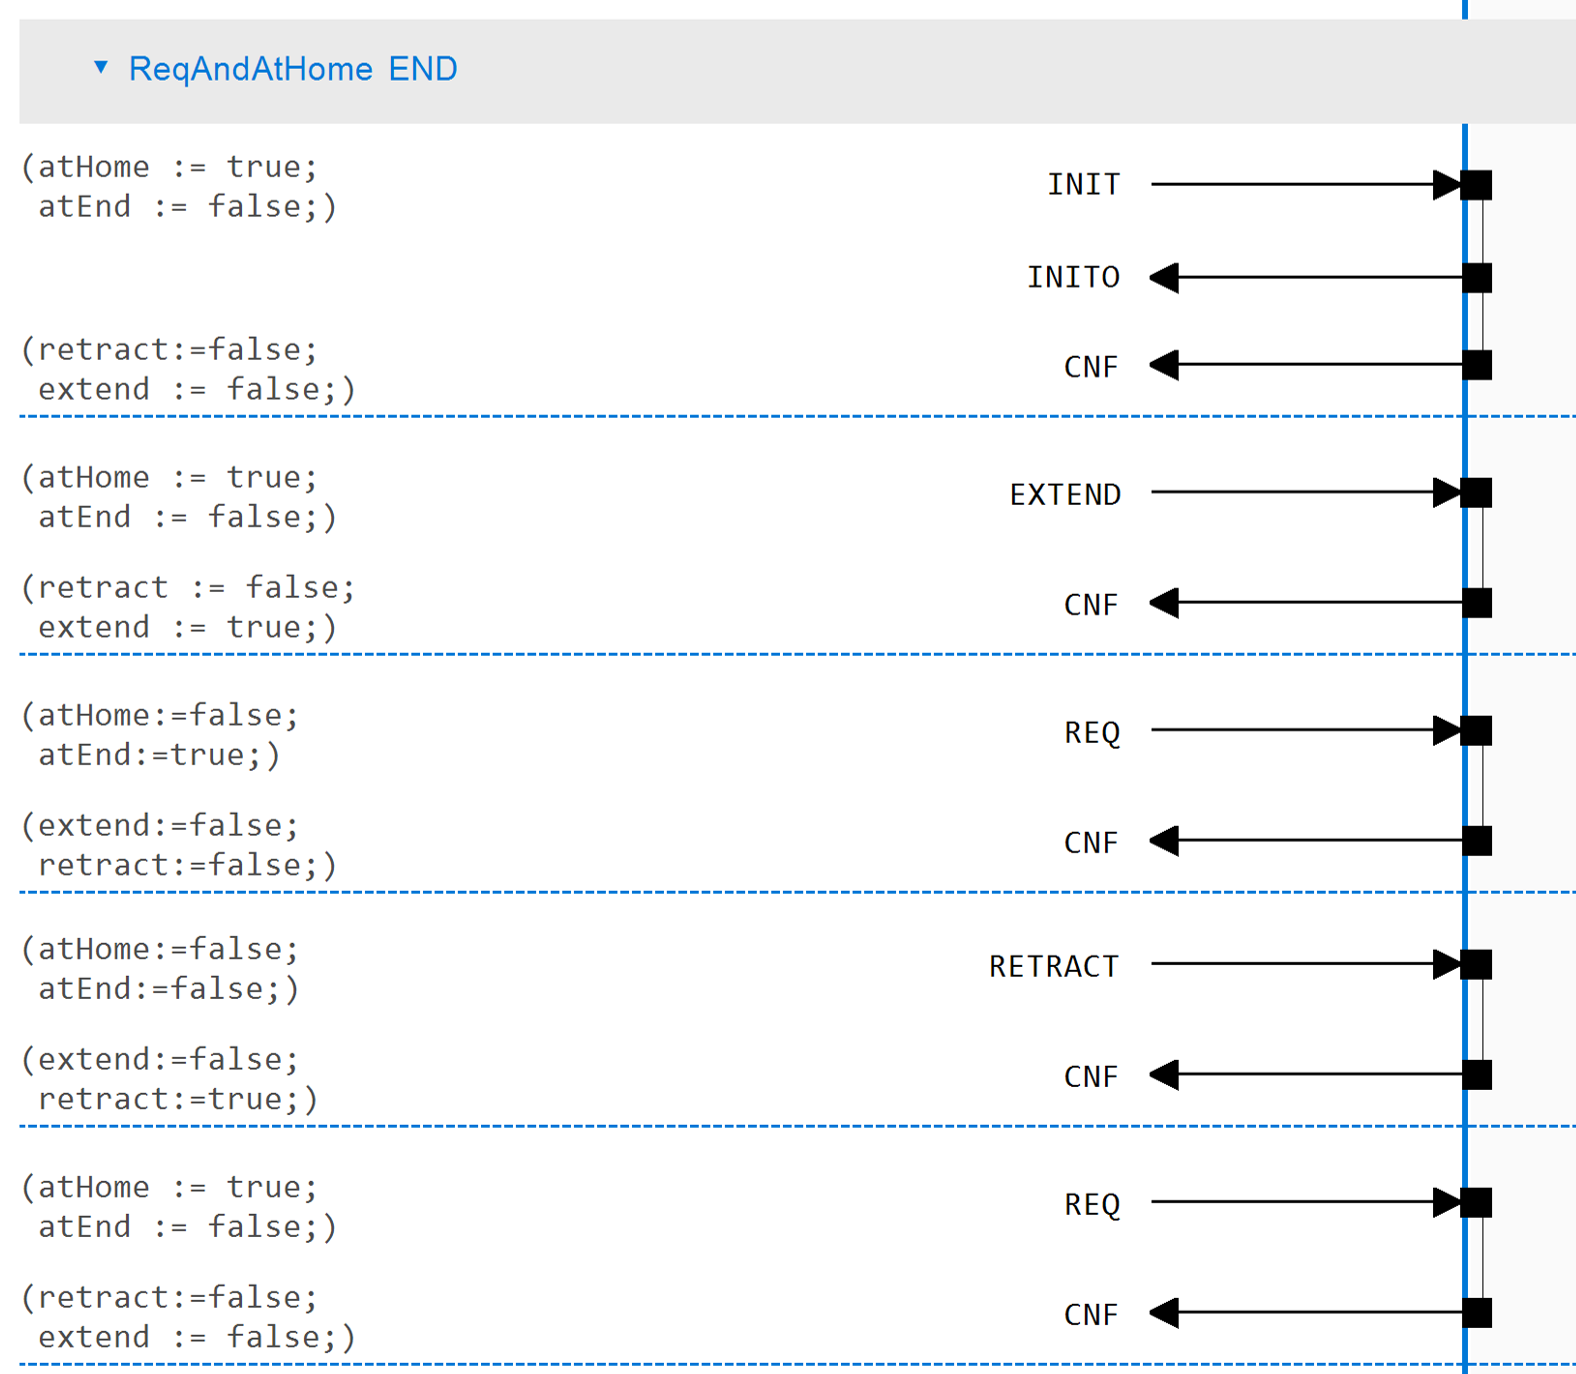
\includegraphics[width=0.99\linewidth]{OJIES_2024/Figures/Service-DoubleActingCylinder_selected.png}
		\caption{Double Acting Cylinder: Interface, state diagram, and selected test cases}
		\label{fig:DoubleActingCylinder}	
 \end{figure}

\section{Evaluation}
We tested the main control FBs from the processing station, but also validated the implementation itself. Following our methodology, we imported any FBs from other tools into 4diac IDE. In 4diac IDE, we then generated the test application, which was executed in 4diac~FORTE and in EcoRT.

\subsection{Evaluating the Generation Framework in Eclipse 4diac}
Selected test cases defined as service sequences as shown in Figures~\ref{fig:TableRotate}, \ref{fig:TestCtrl} and \ref{fig:DoubleActingCylinder}. In total, 12 test cases were created which described both the expected interactions with an FB and deviations (such as events from the environment that occur in a reversed order). To additionally validate that the framework can successfully detect failed test cases, we intentionally defined five service sequences with unexpected behaviour. An example for the TableRotate FB is shown in Figure~\ref{fig:table_rotate_fail}. These experiments validate that the generated test application can indeed detect deviations between the implementation and the specification.

\begin{figure}[hbt]
    \centering
    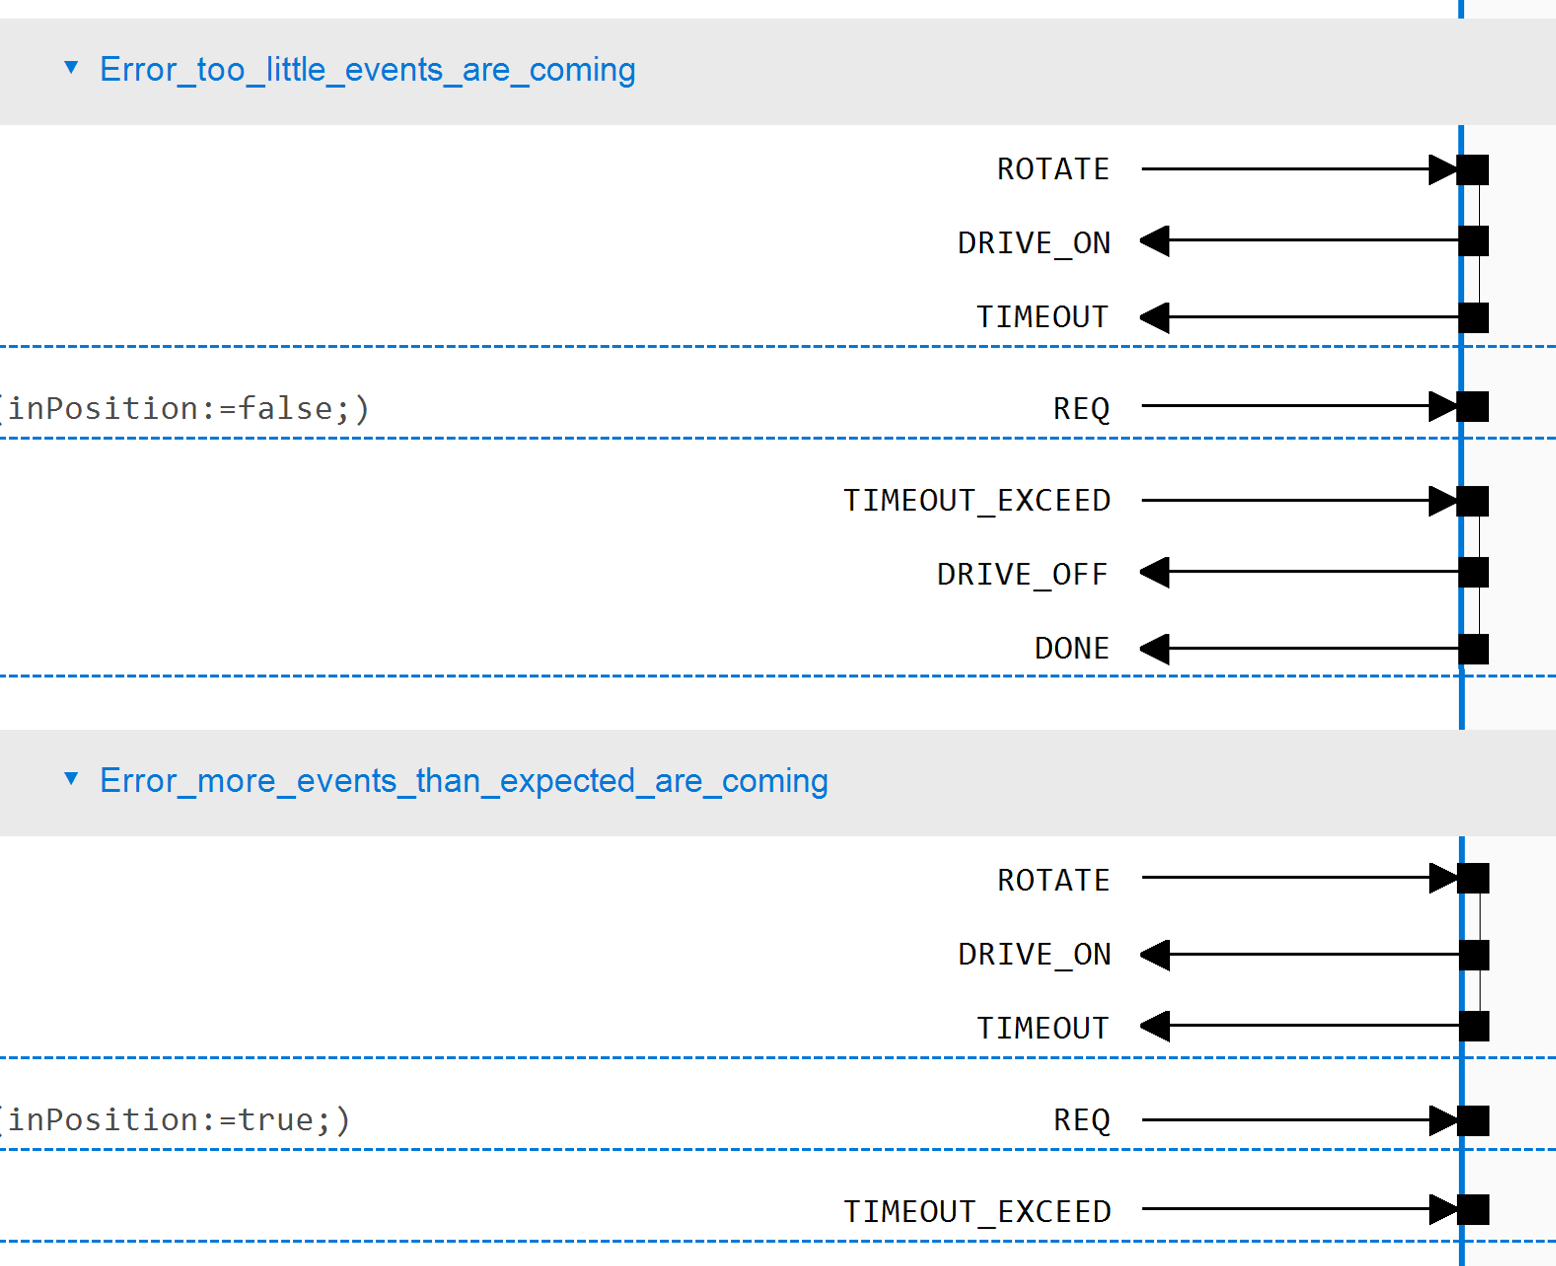
\includegraphics[width=0.7\linewidth]{OJIES_2024/Figures/tests_casestudy/Service-TableRotate_negative.png}
    \caption{Service sequences that result in failed test cases for a correct implementation.}
    \label{fig:table_rotate_fail}
\end{figure}


%We imported the FBs to Eclipse 4diac, defined the tests in its IDE, and generated test applications for them. We also executed the test application on the accompanying runtime 4diac FORTE. After porting the test application to EcoStruxure, we also executed the tests on their runtime environment.

\begin{comment}
\subsubsection{Test case definitions}
Double-acting cylinder
- when it is at home: EXTEND  -> instead of accidentally retract

TestCtrl
- forget to check the sensor value in the ECC

TableRotate
- rotating on/off
- if rotating does not stop after some time, we have a problem (signal inPosition not received -> then it does not stop rotating)
- real example: if you forget to turn a little, the sensor value does not get update


- specify test cases
- introduce faults!?
- try to detect faults with the specified test cases
- report results
\end{comment}

\begin{figure}[h!]
	\centering
		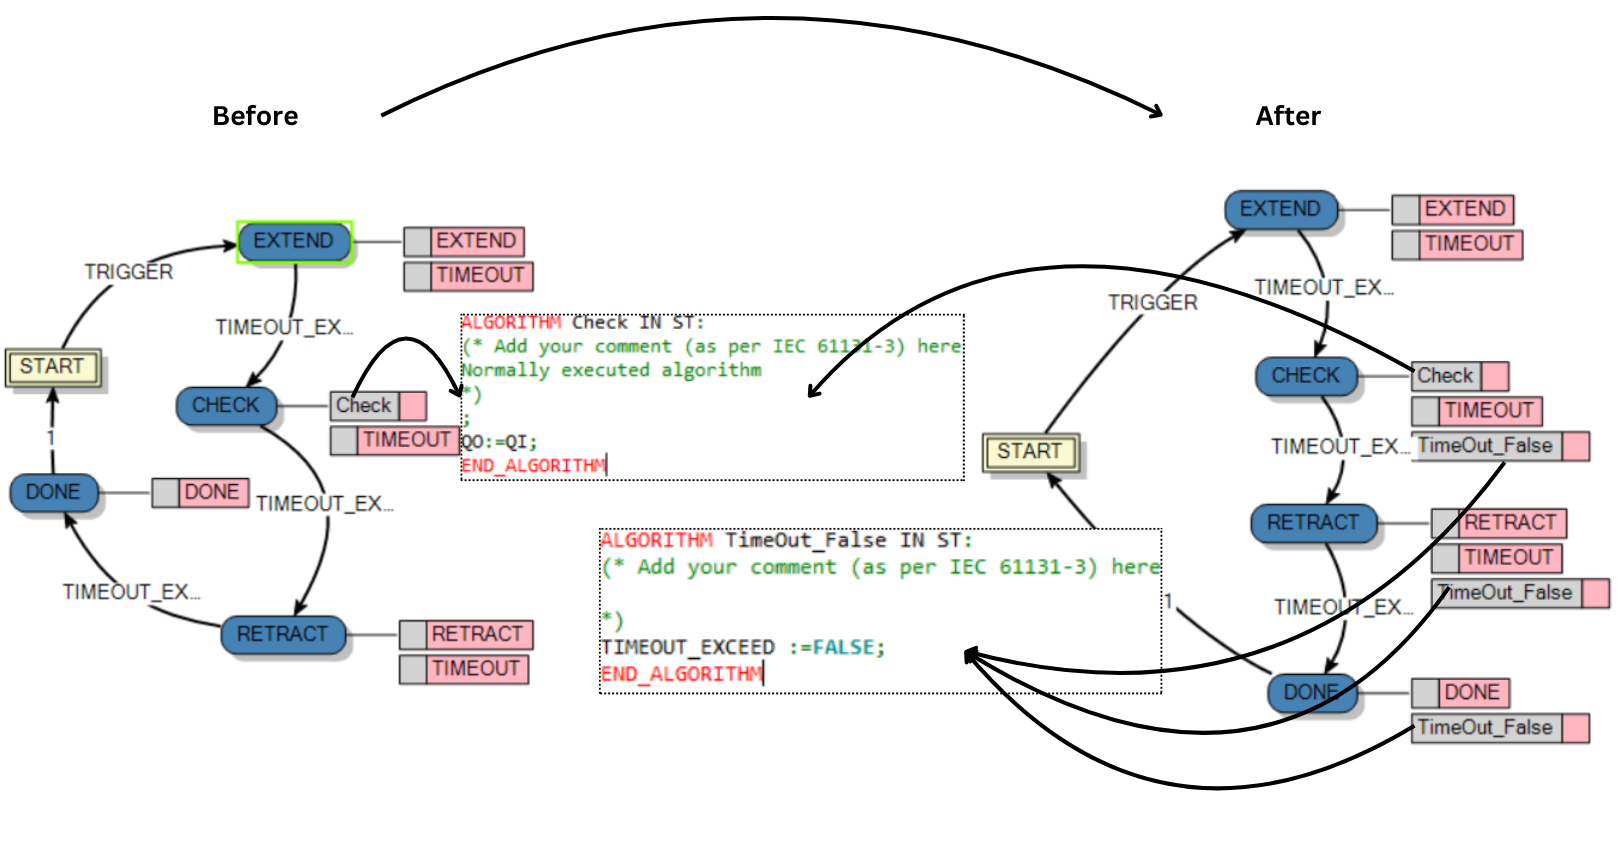
\includegraphics[width=0.99\linewidth,clip]{OJIES_2024/Figures/SemanticExexcissue.png}
		\caption{Semantic Execution issue}
		\label{fig:SemanticExexcissue}	
 \end{figure}

\subsection{Semantic Variants in Ported Software}
All involved FBs were manually imported in a second tool environment to evaluate the behavior of a ported test application. Unfortunately, the testing of FBs on the EcoStruxure Automation Expert (EAE) revealed that certain test cases were failing when executed on the Tester Control. Modifications to the framework were required to compensate the variations in the implemented execution semantics.

Upon thorough analysis, it was determined that these failures were attributed to a semantic execution issue inherent in the EAE. Unlike specified the IEC 61499 standard, EAE adopts a specific semantic execution model. This divergence in execution semantics implies that when a real-world application is ported from Eclipse 4diac to EAE, it may not function correctly, and in some cases, it may even result in system failures.

EAE's semantic execution model operates such that when two or more identical events are used as a sequence of events to transition through multiple states, a single event trigger results in a direct transition to the final state. Specifically, when the event triggers once, the system bypasses intermediate states and directly reaches the final state. 
To illustrate this issue, consider the ECC shown in Figure~\ref{fig:SemanticExexcissue} where the event \texttt{TIMEOUT\_EXCEEDED} is expected to facilitate a sequence of state transitions. According to the desired behavior, upon the first occurrence of the \texttt{TIMEOUT\_EXCEEDED} event, the system should transition to a state labeled \texttt{CHECK}. It should remain in this \texttt{CHECK} state, awaiting a subsequent \texttt{TIMEOUT\_EXCEEDED} event to be triggered before progressing to the final state labeled \texttt{DONE}. However, due to the semantic execution model employed by EAE, when the \texttt{TIMEOUT\_EXCEEDED} event is triggered only once, the system bypasses the \texttt{CHECK} state entirely and directly transitions to the \texttt{DONE} state. This behavior deviates from the intended design, leading to incorrect execution flow.

To address this issue, the test case generation framework was modified to compensate the semantic execution differences. This algorithm modifies the \texttt{TIMEOUT\_EXCEEDED} event by setting its value to \texttt{FALSE}, ensuring that the system remains in the \texttt{CHECK} state after the initial trigger. Consequently, the system only moves to the next state when a subsequent \texttt{TIMEOUT\_EXCEEDED} event is triggered. This modification aligns the execution flow with the expected sequence, preventing premature transitions to the final state.



\section{Results and Discussion}
\label{sec::results}
The semantic differences outlined in the previous section demonstrate the need for a cross-platform testing framework. While the semantic differences could be bridged within our implemented generators, transferring real-world FBs between execution environments can lead to undetected failures. In any portability scenario, this would mean that the distribution of software parts across various vendor's IDEs introduces bugs that are difficult to detect.

It was observed that the control application for our demonstrator contained certain bugs after porting to Eclipse 4diac, which were uncovered during the execution of the test cases. These issues highlight the importance of recognizing the semantic execution differences between EAE and the IEC 61499 standard when porting applications. Addressing such discrepancies is crucial to ensure that applications function as intended within the EAE environment.

The migration of Function Blocks (FBs) from Eclipse 4diac to EcoStruxure Automation Expert (EAE) presents several challenges. Initially, the FBs were imported into 4diac IDE, where tests were defined and test applications were generated. 
These test applications were executed on the accompanying runtime environment, 4diac FORTE. However, when these test applications were ported to EcoStruxure and executed on the EcoRT runtime environment, portability issues arose. The following outlines the key challenges encountered during this migration process.

One significant challenge involves the direct addition of a composite FB containing the \texttt{E\_DELAY} FB. The \texttt{E\_DELAY} FB is a standard function block that is pre-compiled into the vendor's runtime environment. Due to this pre-compiled nature, adding any standard FB directly is not possible. Standard FBs are already available within the vendor's IDE, which necessitates a replacement approach to ensure proper functionality. Consequently, when a composite FB that contains a standard FB is added, it becomes necessary to manually replace the standard FB with an equivalent vendor-provided standard FB within the vendor's IDE. %This manual intervention is crucial to address compatibility issues and ensure seamless integration.

Another issue encountered pertains to adapters and namespaces. In EAE, an adapter cannot be located unless the correct namespace is specified as \texttt{Main}. The definition of the appropriate namespace is essential; otherwise, the adapter will not be displayed. Correcting the namespace can resolve this particular issue. However, even after setting the correct namespace, the use of adapters in composite FBs poses additional problems. These problems require the removal and subsequent redrawing of connections, indicating that the mere correction of namespaces is insufficient when dealing with composite FBs involving adapters.

Further challenges were identified while porting the test FBs in EAE, particularly in relation to the algorithm section within the \texttt{.fbt} file. It was observed that the \texttt{start\_algorithm} and \texttt{end\_algorithm} statements were repeated twice. This redundancy results in errors that must be rectified manually by removing the duplicate statements. Additionally, case sensitivity issues arise within the algorithms. For instance, Boolean variable values are written as \texttt{"false"} and \texttt{"true"} instead of the expected \texttt{"FALSE"} and \texttt{"TRUE"}. This discrepancy requires manual correction to conform to the syntax standards of the target environment.

Another issue relates to the naming conventions used in algorithms. Algorithm names containing double underscores (\texttt{\_\_}) are not supported. As a result, any algorithm names with double underscores must be modified to eliminate this character sequence. This change is necessary to ensure that the algorithms are compatible with the EAE environment. These migration challenges highlight the need for some manual adjustments to ensure the successful transfer and execution of FBs within different automation environments.

\begin{comment}
\begin{table*}[h]
\centering
\begin{tabular}{|l|l|l|l|}
\hline
\textbf{Issue} & \textbf{EAE} & \textbf{4Diac} & \textbf{IEC 61499 Standard} \\ \hline
Direct addition of the \texttt{E\_DELAY} FB is not possible. (Migrating composite FBs with Standard FBs is complex.) & & & \\ \hline
The adapter cannot be found due to the required namespace selection as "Main." & & & \\ \hline
Repeated algorithm definitions and \texttt{end\_algorithm} statements. & & & \\ \hline
Case sensitivity issues in algorithms, e.g., "false" should be "FALSE" and "true" should be "TRUE." & & & \\ \hline
Algorithm names containing double underscores present problems. & & & \\ \hline
The use of "Main::" is not permitted. The namespace should be specified as "Main." & & & \\ \hline
Adapter connection issues require removal and redrawing of connections. & & & \\ \hline
Issues with semantic execution. & & & \\ \hline
Algorithm names containing double underscores present problems, so I changed the names. & & & \\ \hline
\texttt{timeout=false} is written in algorithms. & & & \\ \hline
\end{tabular}
\caption{Migration challenges encountered when transferring Function Blocks (FBs) from 4diac to EAE}
\end{table*}

\subsubsection{other findings}
Did we find any bugs?
Effort reduction?
Problems with different runtimes?
Problems with migration (execution semantics, XML specification)


\end{comment}

In summary, the proposed framework can reduce the effort of porting libraries because the test execution is automated rather than requiring manual labour. 


\section{Limitations}
\label{sec::limitations}
We have proposed and implemented a framework for generating cross-platform tests for IEC~61499-based software. We used two tool environments to evaluate the portability and built on previous results of known execution issues. Currently, no industrial-scale FB libraries are publicly available for testing our approach in practice. As described in the paper, service sequences can serve as test cases for IEC~61499 FBs. However, there is no possibility to specify timing information \cite{Wiesmayr_ifac}. Our approach mainly targets the event-based behaviour of IEC~61499 FBs, while other approaches can cover timing verification (c.f. \cite{Bruns.2023}). 


\begin{comment}
    \item further research on test case generation would be useful
    \item no timing in the 1499 service sequences (e.g., send REQ every 15 ms), hence, also not part of the test generation approach
    \item timing also difficult to test with a test application, but well suitable for the typical problems of 1499 event-based systems
\end{comment}
\section{Conclusion and Future Work}
\label{sec::conclusions}
In conclusion, the proposed testing methodology for IEC 61499 FBs offers systematic and reliable means to verify the correct behaviour of FBs across diverse RTEs. The generation of test FBs from a model-based specification, represented as a service sequence, was accomplished through semi-automated means. Engineers can manually create the test specification (e.g., for test-driven development), or derive it from an existing implementation via the IDE. Our created test FBs are portable across platforms to allow platform-independent testing. This paper presented the overall approach and a first proof-of-concept implementation. We provide an initial set of transformation rules and the corresponding tool support for automating part of the process.

In future work, we aim to support all kinds of FB implementations, provide also the test applications automatically, and evaluate our approach based on a realistic use case to evaluate the scalability and feasibility of the approach in practice. Additionally, developing a runtime comparison tool to analyse and compare the behaviour and performance of FBs across different platforms would enable control engineers to identify and address discrepancies. Finally, integrating the testing approach with further model-based development techniques, such as formal methods or simulation, would provide a holistic approach to system verification and enhance the overall reliability of developed systems.




%% these lines used to import a separate ".bib" for the bibliografy.
\bibliographystyle{bibliography/IEEEtranIES}
\bibliography{bibliography/IEEEabrv,bibliography/mybibfile}

\begin{IEEEbiography}[{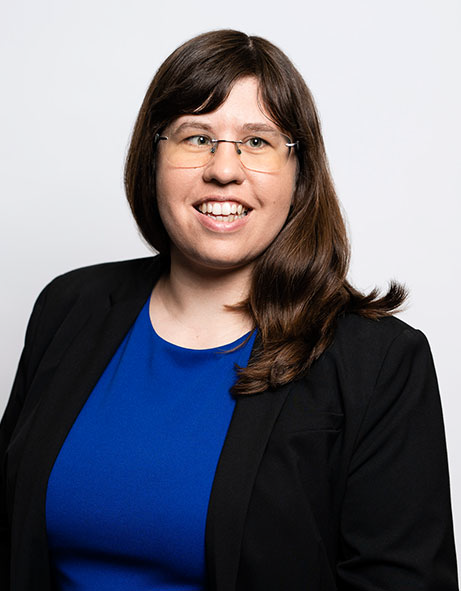
\includegraphics[width=1in,height=1.25in,clip,keepaspectratio]{Figures/photo-bianca.png}}]{Bianca Wiesmayr} is a postdoctoral researcher at the Cyber-Physical Systems Lab at the Linz Institute of Technology (LIT) at Johannes Kepler University (JKU) Linz, Austria. She holds a Master’s degree in Electronics and Information Technology and a doctoral degree in Engineering Sciences from the same university. Her PhD thesis analyzed the use of behavior modeling in the IEC~61499 development process. Her main research interests include model-driven control software engineering as well as modeling tools and their usability.
\end{IEEEbiography}

%%%%%%%%%%%%%%%%%%%%%%%%%%%%%%%%%%%%%%%%%%%%%%%%%%%%%%%%%
\begin{IEEEbiography}[{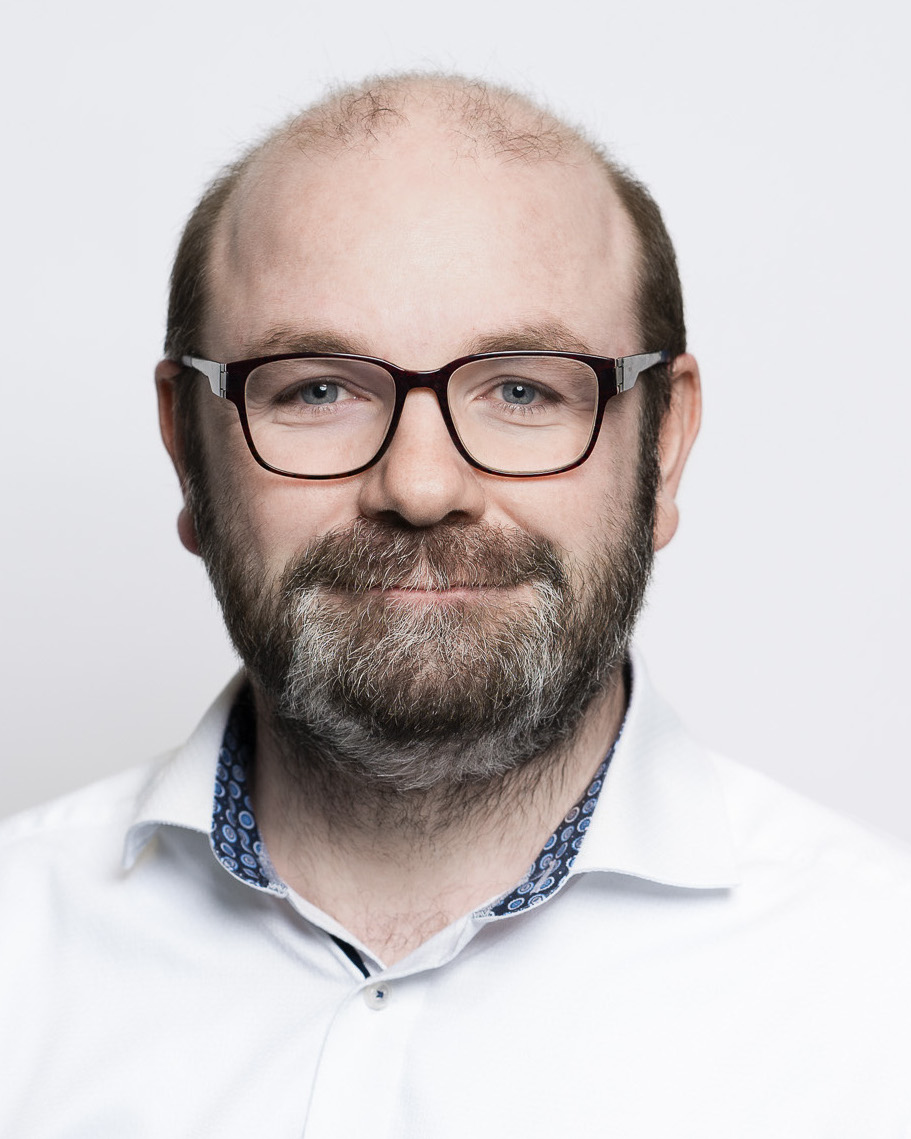
\includegraphics[width=1in,height=1.25in,clip,keepaspectratio]{Figures/Alois_cropped_white_Journal.jpg}}]{Alois Zoitl} (M'08--SM'22) was born in Wels, Austria in 1977. He received the M.S. and PhD degrees in electrical Engineering from Vienna University of Technology, Austria in 2002 and 2007 respectively. 
Since 2018 he is professor of Cyber-Physical Systems for Engineering and Production at the Johannes Kepler University, Linz, Austria.
%He is also part-time with the research institute fortiss in Munich, Germany, where he was leading the competence field Industrie 4.0. 
%Before that he was the head of the research field Distributed Intelligent Automation Systems (Odo Struger Laboratory) at the Automation and Control Institute (ACIN), Vienna University of Technology. 
His research interests are in the area adaptive production systems, distributed control architectures, and dynamic reconfiguration of control applications as well as software development and software quality assurance methods for industrial automation.
He is co-author of more than 200 publications (3 books, 6 book chapters, 19 journal articles) and the co-inventor of 4 patents in the mentioned areas. 
%Alois Zoitl conducted and lead several industry funded R\&D projects as well as coordinated and participated in several public funded (national as well as European) R\&D projects. 
He is a founding member of the open source initiatives Eclipse 4diac, providing a complete IEC~61499 solution, and OpENer. 
%Furthermore, he is a member of the IEEE and GMA. 
Since 2009 he is an active member of the IEC SC65B/WG15 for the distributed automation standard IEC~61499. He was named convenor of the group in May 2015.
\end{IEEEbiography}

\begin{IEEEbiography}[{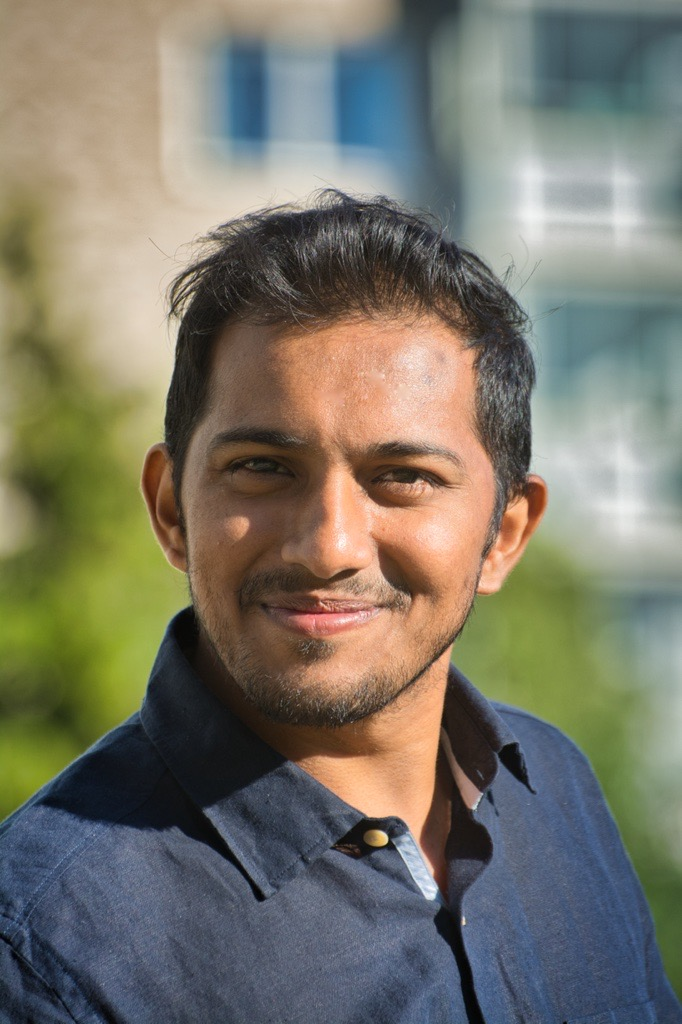
\includegraphics[width=1in,height=1.25in,clip,keepaspectratio]{Bio-Images/midhun.png}}]{Midhun Xavier} received B.Tech in Electronics and Communication Engineering from MG University, Kottayam, India in 2014; the Master of Computer Science from Indian Institute of Information Technology, NIT Trichy Campus, India in 2017. Currently, he is a Ph.D. student at Luleå University of Technology, Luleå, Sweden, with a major in formal verification and modeling of industrial automation systems using IEC 61499 standard. He is also an accomplished software engineer with 3 years of experience in data analytics and web3 development. He has worked with several esteemed organizations such as Uvionics Pvt. Ltd., TCS, and RCKR Software Pvt. Ltd. in India as a Software engineer. 
\end{IEEEbiography}



\begin{IEEEbiography}[{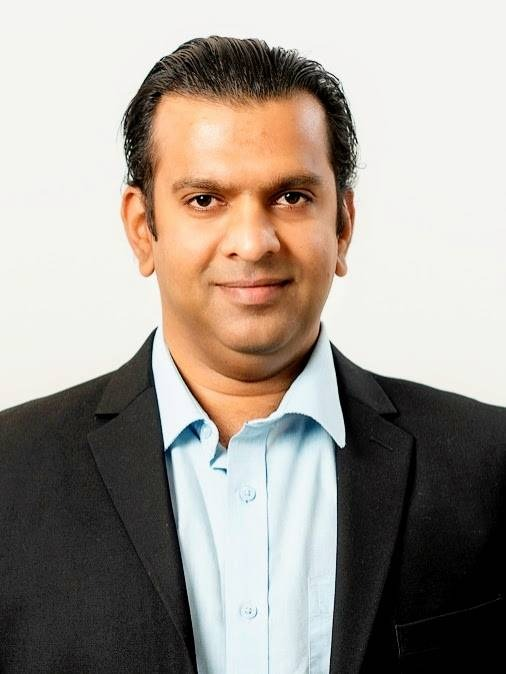
\includegraphics[width=1in,height=1.25in,clip,keepaspectratio]{Bio-Images/sandeep.jpeg}}]{SANDEEP PATIL} (S’11, M’19) received a Bachelor’s degree in computer science engineering from the CMR Institute of Technology, Bangalore, India, in 2005; a Master of computer science (software engineering) degree from the Illinois Institute of Technology, Chicago, IL, USA, in 2010; the Master of Engineering Studies (computer systems) degree from the University of Auckland, Auckland, New Zealand, in 2011; and a Ph.D. degree in formal verification of cyber-physical systems from the Lulea University of Technology, Lulea, Sweden. His research interests include software engineering principles and methodologies in distributed industrial automation, especially using the IEC 61499 paradigm. He also works with formal verification techniques in the same application field. He is an accomplished software engineering professional with over 16 years of research and development experience in systems and application software, including four years as a Senior Software Engineer at Motorola India Pvt. Ltd., India.
\end{IEEEbiography}


\begin{IEEEbiography}[{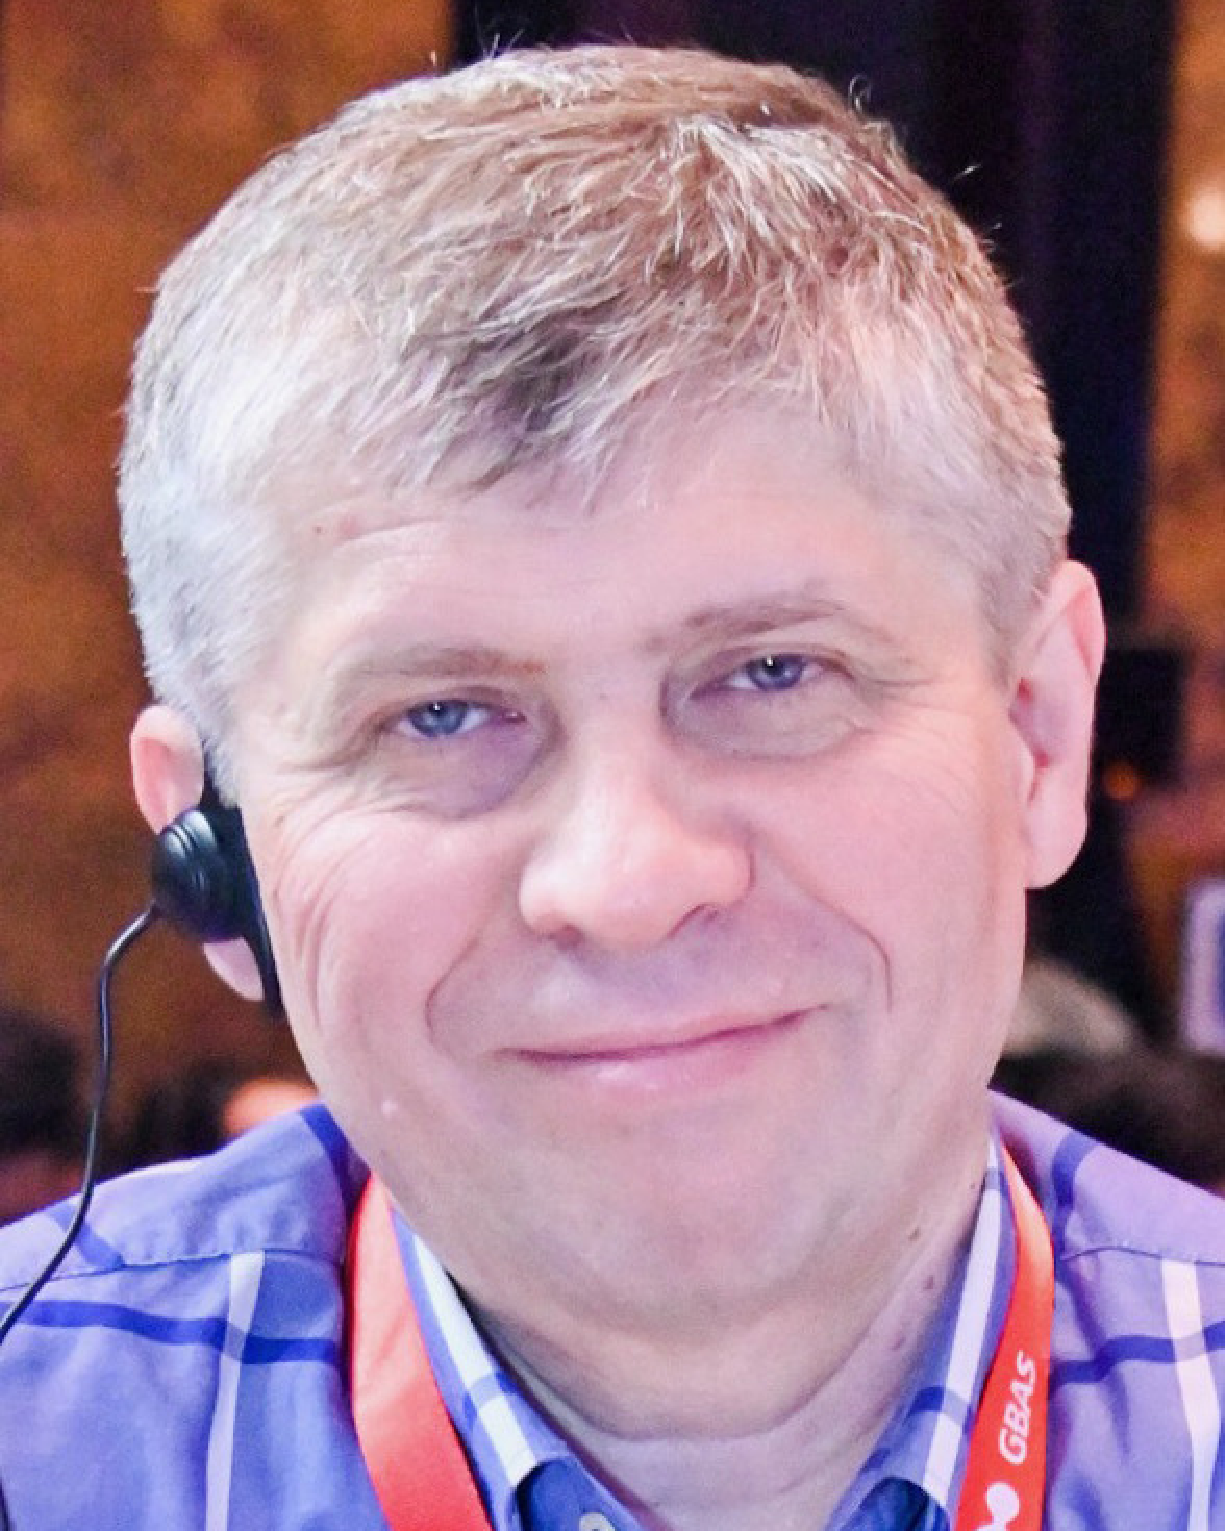
\includegraphics[width=1in,height=1.25in,clip,keepaspectratio]{Bio-Images/vyatk-eps-converted-to.pdf}}]{Valeriy Vyatkin} (Fellow, IEEE) received Ph.D. degrees in Russia and Japan, in 1992 and 1999, respectively, and the Habilitation degree in Germany, in 2002., He is currently on Joint Appointment as the Chaired Professor with the Luleå University of Technology, Luleå, Sweden, and a Full Professor with Aalto University, Helsinki, Finland. Previously, he was a Visiting Scholar at Cambridge University, Cambridge, UK, and had permanent academic appointments with New Zealand, Germany, Japan, and Russia. His research interests include dependable distributed automation and industrial informatics, software engineering for industrial automation systems, artificial intelligence, distributed architectures, and multi-agent systems applied in various industry sectors, including smart grid, material handling, building management systems, data centres, and reconfigurable manufacturing. Dr. Vyatkin was a recipient of the Andrew P. Sage Award for the Best IEEE Transactions Paper in 2012. He has been Chair of the IEEE IES Technical Committee on Industrial Informatics since 2016 and Vice President of IES for Technical Activities for the term 2022–2025.
\end{IEEEbiography}



\EOD
\end{document}
